\documentclass[12pt]{book}
\usepackage[twoside,margin=1in,bindingoffset=0.5in]{geometry}
%\usepackage[round,authoryear]{natbib}
\usepackage{amssymb}
%\usepackage{tocbibind}
\usepackage{graphicx}


\usepackage{amsmath}
\usepackage{listings}
\usepackage{subcaption}
\usepackage[breaklinks = true, linktocpage, pagebackref,
colorlinks = true, hyperindex = true, hyperfigures] {hyperref}
\usepackage[grey]{quotchap}
\usepackage{pdfpages}

\hypersetup{
    colorlinks=false,
    pdfborder={0 0 0},
}

\usepackage{pdflscape}
\usepackage{afterpage}


\renewcommand{\bibname}{Reference List}

\begin{document}
\raggedbottom
%\openup .60em
% Set equal margins on book style
\setlength{\oddsidemargin}{53pt}
\setlength{\evensidemargin}{53pt}
\setlength{\marginparwidth}{57pt}
\setlength{\footskip}{30pt}
\openup 1em
%\includepdf[pages={1}]{titlePDF2}
\frontmatter
%\includepdf[pages={2}]{titlePDF2}
\makeatletter
\chapter{Abstract}

In recent years, there has been a resergence of research and applications within the areas of human computer interaction, these include: virtual reality, augmented reality and 3D reconstruction. This thesis concentrates on the area of 3D reconstruction. In this domain, image and video data is processed to collect 3D structural information. This information has many applications in virtual reality, engineering, architecture and business. Currently, there exist many methods which are capable of extracting 3D structural information from image and video data. Methods include: Feature Matching, Principal Components Analysis and Iterative Closest Point. These algorithms work well in simplistic environments where data noise and corruption is of no concern. Experiments reveal that using Fourier based registration can also recover 3D structural information by registering depth maps. This approach is shown to be robust to noise and object movement. It is capable of solving 1 axis of rotation as well as scale and translation. In cases where 3D rotation must be registered, a novel PCA/Fourier registration methods is proposed. Experiments show that in terms of registration accuracy, this method improves over ICP, feature matching and basic PCA, especially in the presense of noise. During experiments, it was discovered that 3D reconstruction data uses large amounts of storage. 3D data compression methods were also researched. During the PhD, a novel 3D compression method was developed. Results show this outperforms several state of the art methods in terms of low bit rate compression. This is useful for the fourier based registration methods as they are robust to data noise. % Abstract
\makeatletter
\chapter{Acknowledgements}

I would like to thank Dr. Ruben Gonzalez, Dr. Xin-Wen Wu and Dr. Rob Baltrusch for inspiring me. I would particularly like to thank Dr. Ruben Gonzalez for being an excellent supervisor and guiding me in this project.
\tableofcontents
\listoffigures
\listoftables
\mainmatter
item : complete / required

intro : 4/10\\
lit-rev: 40/60\\
meth : 28/60\\
exps : 0/40\\
conc : 0/10\\

total: 98/180\\
refs : 176/200\\



todo:
	finish methodology:
		representations
		sensors
		integrations
		
	programming + write experiments
	do pictures
	re-write intro, results, concl 

\begin{savequote}[8cm]
  ``It is not knowledge, but the act of learning, not possession but the act of getting there, which grants the greatest enjoyment''
  \qauthor{Carl Friedrich Gauss}
\end{savequote}
\makeatletter
\chapter{Introduction}

\section{Introduction}



In recent years, there has been a resergence of research and applications within the areas of human computer interaction, these include: virtual reality, augmented reality and 3D reconstruction. This thesis concentrates on the area of 3D reconstruction. In this domain, image and video data is processed to collect 3D structural information. This information has many applications in virtual reality, engineering, architecture and business. Currently, there exist many methods which are capable of extracting 3D structural information from image and video data. Methods include: Feature Matching, Principal Components Analysis and Iterative Closest Point. These algorithms work well in simplistic environments where data noise and corruption is of no concern. Experiments reveal that using Fourier based registration can also recover 3D structural information by registering depth maps. This approach is shown to be robust to noise and object movement. It is capable of solving 1 axis of rotation as well as scale and translation. In cases where 3D rotation must be registered, a novel PCA/Fourier registration methods is proposed. Experiments show that in terms of registration accuracy, this method improves over ICP, feature matching and basic PCA, especially in the presense of noise. During experiments, it was discovered that 3D reconstruction data uses large amounts of storage. 3D data compression methods were also researched. During the PhD, a novel 3D compression method was developed. Results show this outperforms several state of the art methods in terms of low bit rate compression. This is useful for the fourier based registration methods as they are robust to data noise.

3D Reconstruction research requires the development, testing and analysis of functions which input video and image data and output 3D reconstructed environments. This area is very similar to Simultanious Localization and Mapping or SLAM. However, we have separated the areas as SLAM does not nececarily care about the full dense reconstruction of 3D data. It also has an added requirement of computing localization information. In 3D reconstruction, as long as pleasant, dense and useful 3D reconstructions are computed, localization does not matter.

3D reconstruction is imprortant in a wide variety of areas including business, engineerign and architecture, virtual reality and augmented reality. For example, an architect may want to record 3D structural data in order to study it later. An engineer may want to study the under area of a bridge in order to assess possible faults. Or a software engineer may want to create an augmented reality application where possible home buyers can take virtual tours through an existing property. The scpecifications and 3D structures of these areas may be recorded, in which case 3D models may be built by artists. This however, costs both time and money, furthermore there may be no existing blueprints for the structures, we may also want to provide virtual walking tours through a rainforest, this definately has no blueprint.

Using image and video capturing hardware coupled with 3D reconstruction software, we would be able to scan in an invornmemtn and generate a dense 3D model of it for use in egineering/architectural analysis as well as any kind of virtual reality application. Furthermore, autonomous navigation systems may also generate and use this information as they navigate through a previously unknown environment. Furthermore, with the recent progress made in 3D printing, we may come across a situation where 3D objects and environments may be scanned in using 3D recosntruction and copied via 3D printing.


Without such a system, artists, architects, engineers or scientists would have to build, draw or find some alternative means of generating the 3D data they require. This costs much time and money.

As in other areas of image processing, 3D reconstruction is dominated by feature matching and RANSAC techniques. This involves computing matches between 2D pixels across images, these matches are typically used with RANSAC to compute a camera relationship between the frames. 3D data is then projected and registered using the relationship. This approach is efficient but is not robust to data noise. Furthermore, without some outlier removal function to filter matches, this method fails as feature detection methods typically over-compute matches to the point that only around 30 - 50 percent of features are actually matched. This method also fails in cases where large baselines are used, affine distortion is too large, feature confusion occurs or other times when feature matching fails. Another popular method Iterative Closest Point can be used. This method is more robust to failure than feature matching, and can also be used with RANSAC. However, it fails when the search reaches a local minima in terms of matching error.

Despite the apparent flaws in these methods, they are still popular in both research and industry. In image processing however, alternatives exist. One in particular: Fourier based registration works well at computing 2D rotation, scale and translation. The benefits of this technique are that it is robust to noise and outliers as it takes into account the full signal (it uses the frequency domain to perform fast correlation of data). It is also a closed form sollution (its speed does not depend on the amount of features or on the data itself) and lends itself more easily to parallel processing, a paradime which is set to take over the next generation of software and hardware. Such techniques are frequently used in medical image processing. This raises the question of how well such a technique or related set of techniques would apply to the area of 3D reconstruction.

During the research conducted in quest of answering this question, it was found that the storage and thus manipulation of 3D data became a bottleneck for database and network based operations to do with 3D reconstructed data. To alleviate this issue, compression techniques were also analysed. A set of novel techniques for compression and storage of 3D data are also proposed in this work.  

\section{Research Aims \& Contributions}

The primary aim of this research is to improve the accuracy, noise robustness, speed and storage, quantitative quality and perceptual quality of 3D models. To this end, fourier based registration schemes were investigated as well as compression systems. This motivated the research question, ``Can Fourier based registration techniques improve accuracy and noise robustness in 3D reconstruction applications?'' and ``Can hierarchical techniques improve compression, storage and processing of 3D reconstruction data?'' 

The quest to answer these questions has led to new 3D registration techniques \cite{Lincoln13Interpolating} which outperform ICP and feature matching approaches in terms of noise robustness and accuracy. A novel compression scheme was also developed which was shown to be capable of outperformign existing schemes, this method may be applied to 3D reconstruction storage and retrieval applications and research.

\section{Overview}

Chapter two presents a survey of techniques which may be used for 3D reconstruction. Following this, chapter three introduces some proposed techniques. These are used to answer the research questions and accomplish the primary aim of this project. The fourth chapter details the experiments performed, and presents both quantitative and qualitative results. The fifth chapter contains an analysis of these results and presents findings and discusses results. Finally, the sixth chapter concludes the thesis and discusses the results in terms of the primary aim and research question. 


 % The Introductory Chapter
\input{chapters/literatureReview} % The Literature Review
\begin{savequote}[8cm]
  ``I have not failed. I've just found 10,000 ways that won't work.''
  \qauthor{Thomas Edison}
\end{savequote}
\makeatletter
\chapter{Methodology}

\section{Introduction}

Here we present several techniques used to extract dense 3D reconstruction from image/video data. In the first section we describe techniques in addition to Fourier volume registration. These include the recovery of translation, y-axis rotation and scale information as well as a technique for the recovery of a so called 7 degrees of freedom transform. \\

We also list notable speed-ups for volume registration which reduce the amount of processing by over a third. After this, a full 3D reconstruction technique based on the principles of phase correlation is presented. Then we also present two novel reconstruction data representations which may be used to efficiently represent and fuse 3D reconstructions. Lastly, different sensor inputs are discussed and some conclusions are given about the usefulness of this technique in the context of these sensors is presented.

\section{Fourier Volume Registration} 

\subsection{Recovery of Translation Values}

Given a volume $V_1$ and a spatially shifted version of it $V_2$, the offset along each axis, $(x,y,z)$ may be recovered if a suitable correlation between the two volumes can be found. \\

The measure of correlation between $V_1$ and $V_2$ can be found by shifting $V_1$ and $V_2$'s mean values to zero, then summing the element-wise multiplication of $V_1$ by $V_2$. Equation \ref{eqn:CorrelationEquation} computes this correlation measure.

\begin{equation} \label{eqn:CorrelationEquation}
\sum_{z=0}^{N}\sum_{y=0}^{N}\sum_{x=0}^{N}(V_1(x,y,z)-avg(V_1)) \times (V_2(x,y,z)-avg(V_2))
\end{equation}

Using this measurement, two volumes which are similar in signal shape (element-wise-value to location correspondence) will give a larger measure of correlation than two volumes with a differing signal shape. If the volumes are first normalized we can regard volume $x$ is more aligned with volume $y$ than with volume $z$ given $x$ correlated with $y$ gives a larger value than $x$ correlated with $z$. \\

Cross-correlation searches over a space of translation parameters and outputs the optimal translation to align two volumes. It is optimal in the sense of correlation measurement. This is used as a best guess in terms of the alignment of the two volumes. It can be thought of as the optimization of parameters $x,y,z$ in equation \ref{eqn:CrossCorrelationEquation}.

\begin{equation} \label{eqn:CrossCorrelationEquation}
CrossCorrelate(Transform(V_1, x,y,z), V_2)
\end{equation}

Since we typically do not know the range of translation values $x,y,z$ to optimize for, we take into account the range from $[0,N]$ where $N$ is the width/height/depth of the volume. This gives a complexity of $N^6$. This is too computationally complex for practical volume sizes. Therefore, we use the properties of the Fourier Transform to reduce computational complexity. \\
 
The 3D Fourier transform transforms a volume from the 3D spatial domain into the 3D frequency domain. The frequency domain is a complex valued volume made up of sinusoids where each value in the frequency domain represents the magnitude, phase and direction of a wave.  \\


WARNING: show picture of 3D volume fft\\

WARNING: show picture of 3D pc surface\\

Using the properties of the Frequency domain, we can efficiently recover the optimal alignment translation parameters using a function called $PhaseCorrelation$ (Eq. \ref{eqn:PC_basic}). This function takes two volumes as input and returns the best alignment translation between them in terms of maximizing correlation.
\begin{equation} \label{eqn:PC_basic}
(x, y, z) = PhaseCorrelation(V_x, V_y)
\end{equation}
The $PhaseCorrelation$ function first applies 3D FFTs to volumes, $V_1$ and $V_2$, converting them into the frequency domain, i.e. $F_{1_{x,y,z}} = FFT(V_1)$ and $F_{2_{x,y,z}} = FFT(V_2)$. Taking the normalised cross power spectrum using Eq. \ref{eqn:PHCOR_eq} based on these frequency domain volumes computes the frequency domain of a new volume called the phase correlation volume. \\


\begin{equation} \label{eqn:PHCOR_eq}
F_{3_{x,y,z}} = \frac{F_{1_{x,y,z}} \circ F_{2_{x,y,z}}^*}{ | F_{1_{x,y,z}} \circ F_{2_{x,y,z}}^* | }
\end{equation}

Here, $\circ$ is an element-wise multiplication and $|x|$ is the magnitude function. Taking the inverse FFT of the frequency domain of the phase correlation volume, $F_3$ gives the phase correlation volume itself, $V_3$ ($V_3 = FFT^{-1}(F_3)$). The location of the peak value in the phase correlation volume $V_3$, $(x_1, y_1, z_1)$ gives the shift between the $V_1$ and $V_2$. The phase correlation volume is typically noisy making the peak difficult to locate. Each in the phase correlation volume evaluates the correlation between $V_1$ (translated by the location of the peak) and $V_2$.


\subsection{Recovery of Y-Axis Rotation and Scale}

Using the phase correlation procedure along with some spatial transformation functions allows the computation of a single axis of rotation (out of 3) along with the scale difference between two volumes. If $V_1$ and $V_2$ are translated, rotated and scaled versions of the same volume, such that they are related by some translation $(t_x, t_y, t_z)$, y-axis rotation $\theta$, and scale $\varphi$.\\


WARNING: show picture of log-spherical transform\\

Here we describe how to compute the rotation and scale parameters, further action is required to recover translation. The first step, given two volumes $V_1$ and $V_2$ of size $N^3$ is to apply a Hanning windowing function (Eq. \ref{eqn:Hann}). This function assists in filtering the volumes prior to a discrete Fourier transform being applied to them. Since the discrete Fourier transform relies on a continuous signal (volume) and this cannot be used in the calculation, by reducing the signal strength near the volume borders, we can improve the accuracy of the discrete Fourier transform.
\begin{equation} \label{eqn:Hann}
\scriptstyle
HW_{x,y,z} = \frac{1}{2}\left(
1 - cos \left(
\frac{2\pi
\left(
\sqrt{\left(\frac{N}{2}\right)^3} -
\sqrt{
\left(x-\frac{N}{2}\right)^2 + \left(y-\frac{N}{2}\right)^2 + \left(z-\frac{N}{2}\right)^2
}
\right)
}
{2\sqrt{\left(\frac{N}{2}\right)^3} - 1}
\right)
\right)
\end{equation}
The rotation and scale factors can only be recovered if translation information is removed from the two volumes. Therefore we take the magnitude of the FFT of the volumes, $M_1 = |FFT(V_1)|$, $M_2 = |FFT(V_2)|$. Since the magnitude values do not contain phase information they do not, by nature, contain location information of the volume (translation information). The zero-frequency of both $M_1$ and $M_2$ is next shifted to the center of the volume and the log of the result is taken $M'_1 = Log(M_1)$, $M'_2 = Log(M_2)$. Like in phase correlation the log function spreads out the contribution of the frequencies so that high frequencies contribute as much as lower frequencies which have larger magnitudes. A log-spherical transform is then used to turn rotation and scaling into translation for both $M'_1$ and $M'_2$. Eq. \ref{eqn:Log_Spherical} shows the corresponding log-spherical space coordinate $(X_{log-spherical}, Y_{log-spherical}, Z_{log-spherical})$ for a given $(x,y,z)$ euclidean space coordinate.
\begin{equation} \label{eqn:Log_Spherical}
\begin{split}
X_{log-spherical} & = \frac{atan\left(
\left(\frac{x-\frac{N}{2}}{\sqrt{x^2+y^2+z^2}}\right)
\left(\frac{y-\frac{N}{2}}{\sqrt{x^2+y^2+z^2}}\right)^{-1}
\right)N}{360}\\
Y_{log-spherical} & = \frac{acos\left(
\frac{y}{\sqrt{x^2+y^2+z^2}}
\right)N}
{180} \\
Z_{log-spherical} & =\frac{log\left(\sqrt{x^2+y^2+z^2}\right)N}{log\left( \frac{N}{2.56} \right)} \\
\end{split}
\end{equation}
The log-spherical transforms of $M'_1$ and $M'_2$ are then phase correlated to find the shift between them, $(x_{M'},y_{M'},z_{M'}) = PhaseCorrelation(M'_1, M'_2)$. The rotation $\theta$ and scale $\varphi$ factors between $V_1$ and $V_2$ can then be found from the shift parameters using Eq. \ref{eqn:ROTATIONSCALEFROMXM} . 
\begin{equation} \label{eqn:ROTATIONSCALEFROMXM}
\begin{split}
\theta & = \frac{-360x_{M'}}{N}\\
\varphi & = e^{
-\left(
2.56^{-1}N
\right)z_{M'}N^{-1}
}
\end{split}
\end{equation}
Using $\theta$ and $\varphi$, $V_1$ can now be inverse transformed (using $(\frac{N}{2}, \frac{N}{2}, \frac{N}{2})$ as the origin). This aligns $V_1$ and $V_2$ with respect to scale and y-axis rotation. The translation parameters $(t_x, t_y, t_z)$ can then be found using phase correlation as given in Eq. \ref{eqn:FINALTRANS}.
\begin{equation} \label{eqn:FINALTRANS}
(t_x, t_y, t_z) = PhaseCorrelation(scale(rotate(V_1,\theta),\varphi), V_2)
\end{equation}
The complete function to recover translation, rotation and scaling, combining equations \ref{eqn:PHCOR_eq}-\ref{eqn:FINALTRANS} as is denoted in \ref{algorithm:PCSLAM} is \ref{eqn:FULLPC}.
\begin{equation} \label{eqn:FULLPC}
(\theta, \varphi, t_x, t_y, t_z) = PhaseCorrelation_{\theta \varphi t_x t_y t_z}(V_m, V_n)
\end{equation}

\subsection{Full Recovery of 3D Rotation}

\label{FullRecovery3DSection}

In order to recover full 3D rotation (as well as scale and translation) the model must first be aligned by some common axis. PCA or Principals Component Analysis is a well known technique for recovering the primary axes of an N-dimensional signal. In this case, we can use the most accurate axis (the eigen-vector with the largest corresponding eigen-value) to align two volumes, then y-axis rotation, scale and translation values can be recovered by the described FFT based volume registration method. \\

WARNING: SHOW picture of this PCA procedure

PCA is a capable registration technique on its own, but when faced with non-overlapping, missing or noisy data it typically fails on its own. The technique of alignment is discussed in the following sections. \\

Given a 3-dimensional signal $A$ of length $N$, the co-variance of the signals between two of the dimensions ($x$ and $y$) is given as a function in equation \ref{eqn:Covariance3DSignal}.

\begin{equation} \label{eqn:Covariance3DSignal}
Cov(A_x,A_y) = \sum_{i=0}^{N}(A_{x_i} - A_{x_{mean}})(A_{y_i} - A_{y_{mean}})
\end{equation}

Here, $A_{x_{mean}}$ and $A_{y_{mean}}$ are the mean values of these x and y dimensions of $A$. 

Using the voxel locations of volume $A$ we can generate the covariance matrix \ref{eqn:CovarMatrix}. This matrix describes the how each coordinate changes with respect to each other.

\begin{equation} \label{eqn:CovarMatrix}
\left[
\begin{array}{ccc}
Cov(A_x, B_x) & Cov(A_x, A_y) & Cov(A_x, A_z) \\
Cov(A_y, B_x) & Cov(A_y, A_y) & Cov(A_y, A_z) \\
Cov(A_z, B_x) & Cov(A_z, A_y) & Cov(A_z, A_z) \\
\end{array}
\right]
\end{equation}

The 3 eigen-vectors of the covariance matrix describe the primary axis of the signal $A$ and the 3 corresponding eigen-values describe the strength of these axes. The eigen-vector/axis with the largest corresponding eigen-value is the principal component. The principal component is used to align data to a common axis. Here we define the principal axis (component) of a 3D signal $A$ as $A_{pa}$. \\

Given a 3D volume $V$, with a computed principal axis $V_{pa}$ and mean $V_{mean_location}$, we can construct a matrix to normalize the 3D data in terms of the principal axis.

Given $V_{pa}$ a vector pointing along the principal axis of $V$, we compute the forward vector as 


\begin{equation} \label{eqn:fwdVector}
Fwd = \left(\left[
\begin{array}{c}
V_{pa_{x}}\\
V_{pa_{y}}\\
V_{pa_{z}}\\
\end{array}
\right] \times \left(\left[
\begin{array}{c}
1\\
0\\
0\\
\end{array}
\right] \times \left[
\begin{array}{c}
V_{pa_{x}}\\
V_{pa_{y}}\\
V_{pa_{z}}\\
\end{array}
\right]\right)\right) \times \left[
\begin{array}{c}
V_{pa_{x}}\\
V_{pa_{y}}\\
V_{pa_{z}}\\
\end{array}
\right]
\end{equation}

Here, $\times$ is the cross-product of the vectors. The right pointing vector is computed as orthogonal to the forward vector and the common vertical axis $V_{pa}$,


\begin{equation} \label{eqn:fwdVector}
Rgt = \left[
\begin{array}{c}
V_{pa_{x}}\\
V_{pa_{y}}\\
V_{pa_{z}}\\
\end{array}
\right] \times \left[
\begin{array}{c}
Fwd_x\\
Fwd_y\\
Fwd_z\\
\end{array}
\right]
\end{equation}

Then the volume can be normalized to an axis based on the input data. This is done using a matrix which transforms the data to the origin, then corrects the vector $V_{pa}$ to be the new up axis, then transforms back. The matrix in equation \ref{eqn:CorrectUpMat} computes this,


\begin{equation} \label{eqn:CorrectUpMat}
CorrectMat(V) = \left[
\begin{array}{cccc}
1 & 0 & 0 & V_{mean_x} \\
0 & 1 & 0 & V_{mean_y} \\
0 & 0 & 1 & V_{mean_z} \\
0 & 0 & 0 & 1 \\
\end{array}
\right] \left[
\begin{array}{cccc}
Rgt_x & Rgt_y & Rgt_z & 0 \\
V_{pa_x} & V_{pa_y} & V_{pa_z} & 0 \\
Fwd_x & Fwd_y & Fwd_z & 0 \\
0 & 0 & 0 & 1 \\
\end{array}
\right] \left[
\begin{array}{cccc}
1 & 0 & 0 & -V_{mean_x} \\
0 & 1 & 0 & -V_{mean_y} \\
0 & 0 & 1 & -V_{mean_z} \\
0 & 0 & 0 & 1 \\
\end{array}
\right]
\end{equation}


To recover a matrix for full 3D rotation, scale and translation for given volumes $Volume_A$ and $Volume_B$, we first compute the correction matrices using PCA and the technique described above for both $Volume_A$ and $Volume_B$ as $C_A = CorrectMat(Volume_A)$ and $C_B = CorrectMat(Volume_B)$. The transformation matrix relating $Transform(Volume_A, C_A)$ and $Transform(Volume_B, C_B)$ is computed as $RST$. The final transform then relating $Volume_A$ to $Volume_B$ is computed as,

\begin{equation} \label{eqn:FullRSTTransform}
R_{x,y,z}ST Matrix = C_{B}^{-1} \times RST \times C_A
\end{equation}

This technique is capable of extending Fourier registration to take into account full 3D rotation. The technique simply requires a single iteration over the data to compute the principal components then a rotation-scale-translation phase correlation technique is used to compute the scale, translation and y-axis rotation. 

WARNING: show an example of this working

\subsection{Filtering Techniques}

\subsection{Fast Fourier Volume Registration}

3D phase correlation is CPU and GPU intensive, so in order to reduce complexity we tried to minimize processing in areas which require the most computation time. In out Fourier based volume registration method defined in the previous section, this occurs in the two 3D phase correlations which need to be computed. We describe the method of reduction here; a block diagram for this technique is given in figure \ref{fig:PIPELINE3} WARNING:Given a picture for the sped up version too!. We refer to this method as fast volume registration (FVR) in reference to general volume registration (VR). The speedup begins by computing the 3D DFT of both input volumes and taking the magnitude of these. Rather than directly performing a 3D log-spherical transform and a 3D phase correlation operation on these volumes, we use a novel transform we call a spherical-map transform (details in \ref{SMTransform}).\\

\begin{figure*}[t]
\centering
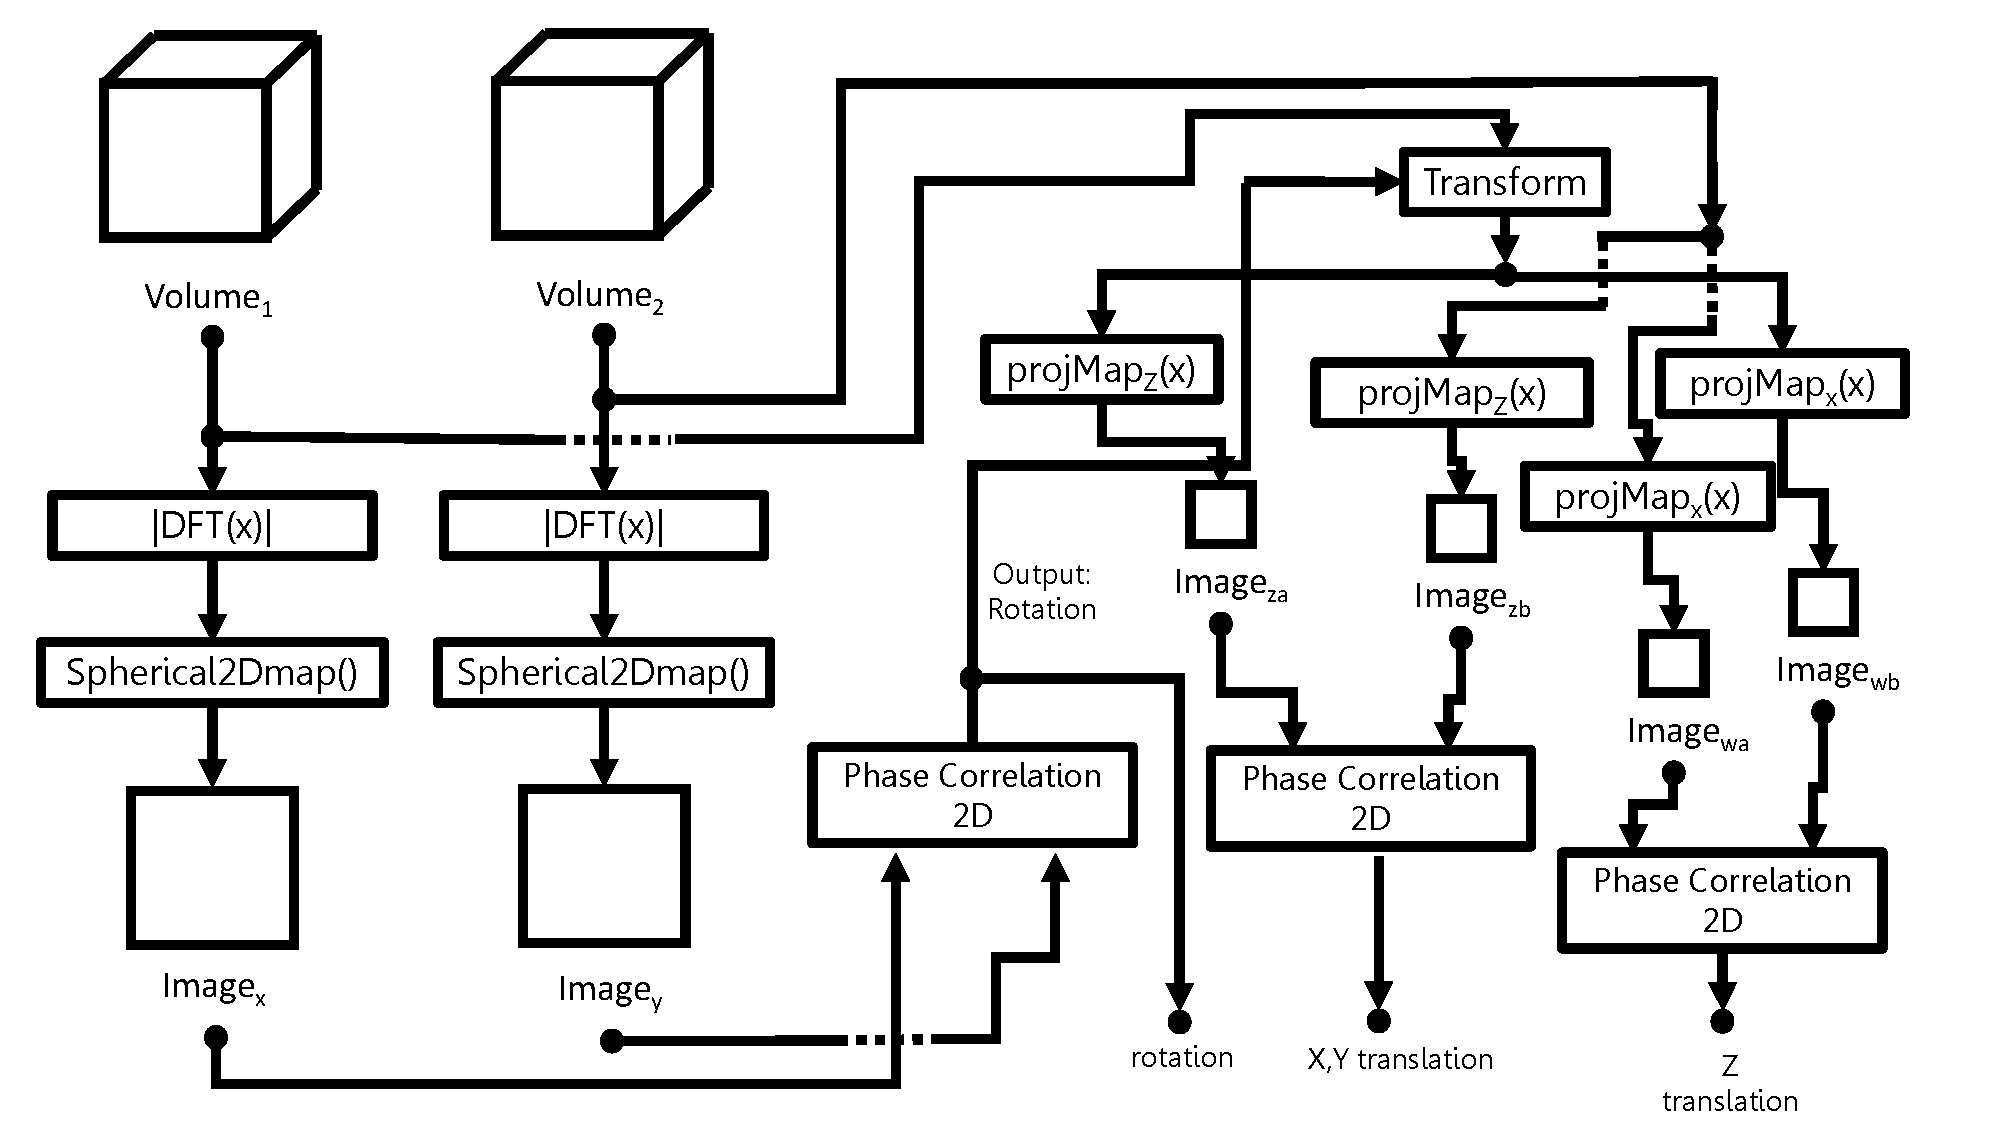
\includegraphics[width=6.0in]{images/ch2/pipeline3}
\caption{System Diagram for Fast Volume Registration}
\label{fig:PIPELINE3}
\end{figure*}

This transform converts rotation into translation whilst simultaneously unfolding the 3D space down to 2-dimensions. After this, a 2D phase correlation that requires significantly less processing compared with the 3D counterpart is used to compute the rotation. Next, having obtained the rotation parameter, the rotation is eliminated from the transformation by rotating the first volume by this parameter. The two volumes are then passed through two orthogonal projection mapping functions. This also converts the volumes to 2D space. We use two transforms for both volumes, one projection along the x-axis, another along the z-axis. Once the x-axis projections of both volumes are complete, we can do another 2D phase correlation to give us the z-translation. The 2D phase correlation of the z-axis projections gives us the x and y axis translations separating the original volumes. The final output of this method gives the rotation and translational shifts between the input volumes. The projections add little complexity to the overall algorithm and since 2D phase correlation operations are used in place of 3D ones, much computation time is reduced.

\subsection{Spherical-map transform}
\label{SMTransform}
The spherical map transform both reduces the 3D volume to a 2D image, and any rotation about the y-axis becomes x-axis translation in the output image. An example of the bunny model and the spherical-map transform of this model is given in figure \ref{fig:smtExample}, the mathematics are defined in equations \ref{eqn:invLPFuncs} and \ref{eqn:smtUpdate}. Given a coordinate in 2D Cartesian space x,y, we compute the ray $[Ray_x Ray_y Ray_z]^T$ from the volume center and sum up the voxel values along the ray (equation \ref{eqn:smtUpdate}). \\


\begin{equation} \label{eqn:invLPFuncs}
\begin{split}
Ray_x(x,y) & = cos\left(\frac{360x}{N}\right)sin\left(\frac{180y}{N}\right)  + \frac{N}{2} \\
Ray_y(y) & = cos\left(\frac{180y}{N}\right) + \frac{N}{2} \\
Ray_z(x,y) & = 	sin\left(\frac{360x}{N}\right)sin\left(\frac{180y}{N}\right) + \frac{N}{2}
\end{split}
\end{equation}

\begin{equation} \label{eqn:smtUpdate}
Im_{x,y} = \sum_{r=1}^{(2^{-1}N)^{1.5}}{Vol(Ray_x(x,y)r, Ray_y(y)r, Ray_z(x,y)r)} 
\end{equation}

This process essentially sums up the values along a given ray defined by scaling spherical coordinates and adding up the values intersecting the ray. The resulting image, maps 3D y-axis rotation to 2D x-axis translation.  \\

\begin{figure*}[t] 
        \centering
        \begin{subfigure}[b]{4.2in}
                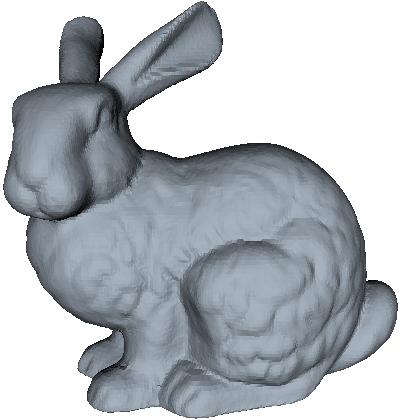
\includegraphics[width=4.2in]{images/ch2/bunny}
                \caption{original}
                \label{fig:bunnyOrig}
        \end{subfigure}
        \begin{subfigure}[b]{4.2in}
                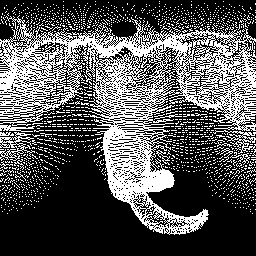
\includegraphics[width=4.2in]{images/ch2/spherical2DMap}
                \caption{transform}
                \label{fig:bunnySPTed}
        \end{subfigure}%
        \caption{The Spherical Map Transform.}
       \label{fig:smtExample}
\end{figure*}


\subsection{Projection-map transform}

The projection map transform is similar to an orthogonal projection of the volume along some given axis. For the projection map transform, given an output image $Im_a$ and an input volume $Vol_a$, each pixel in $Im_a$ is defined mathematically as the summation of values along a particular axis given the image coordinates. The x-axis transform and the z-axis transform are defined in equations \ref{eqn:xPMT} and \ref{eqn:zPMT} respectively. \\

WARNING: add in a picture here

\begin{equation} \label{eqn:xPMT}
Im(z,y) = \sum_{x=0}^{N}{Vol_a(x,y,z)}
\end{equation}

\begin{equation} \label{eqn:zPMT}
Im(x,y) = \sum_{z=0}^{N}{Vol_a(x,y,z)}
\end{equation}

The process defined by equation \ref{eqn:xPMT} maps 3D z-axis translation to 2D x-axis translation, whilst equation \ref{eqn:zPMT} maps 3D x-axis and y-axis translation into 2D x-axis and y-axis translation.


To assess the performance of our method, the size of the volumes being registered is defined as $N^3$ whilst each frame is sampled at a resolution of $W$ $\times$ $H$. The projection process requires $12WH$ operations whilst re-sampling the point cloud requires $2WH$ operations. The Volume Registration process, $VolumeRegister{\theta \varphi t_x t_y t_z}(V_1, V_2)$ consists of 2 $\times$ Hanning windowing processes, 2 $\times$ 3D FFTs, 2 $\times$ volume-logs, 2 $\times$ log-spherical transforms, 2 $\times$ phase correlation processes and 1 $\times$ linear transformation and peak finding. 

The Hanning windowing function requires 26 operations. The 3D FFT has complexity of $3N^3\log{N}$, the log and log-spherical transform functions require 3 and 58 operations per voxel respectively. Multiplying two frequency spectra together and transforming a volume requires 15 and 30 operations per voxel respectively. Finding the peak value requires $2N^3$ operations. The complexity in terms of number of operations for the phase correlation process is given in Eq. \ref{eqn:PCFULLPERFORMANCE} This process requires 2 $\times$ 3D FFTs, 1 $\times$ frequency spectra multiplication, and 1 $\times$ peak finding operation. 
\begin{equation} \label{eqn:PCFULLPERFORMANCE}
6N^3\log{N} + 2N^3 + 15
\end{equation}
The total complexity can then be found by taking into account the projection and re-sampling totals as well as the total for $VolumeRegister{\theta \varphi t_x t_y t_z}(V_1, V_2)$. Tallying the number of operations for each process and multiplying them by number of times the process is performed gives us the number of operations as a function of $W$, $H$ and $N$ in Eq. \ref{eqn:FULLPERFORMANCE}.
\begin{equation} \label{eqn:FULLPERFORMANCE}
6N^3 + 28WH + 18(N^3\log{N}) + 230
\end{equation}



To compare performance of the generic volume registration method with the speed up, we use the complexity defined in equation \ref{eqn:FULLPERFORMANCE}. Here, we ignore the cost of projecting the depth map. The 3D DFT has complexity $3N^3log(N)$. This is the first step (see figure \ref{fig:PIPELINE3}), the next is the spherical-map transform which is complexity $45N^3$. If processed on the GPU the performance becomes 45 operations per voxel assuming that one voxel is assigned to one unit of processing. A 3D transform is 30 operations per voxel, 2D phase correlation requires 15 operations to multiply the frequency spectra and $2N^2log(N)$ operations to do the 2D FFT. Finally a projection map transform requires 1 operation per voxel. \\

In total, the proposed method requires $2 \times$ 3D FFTs, $2 \times$ spherical-map transforms, $1 \times$ 3D geometrical transformation, $3 \times$ 2D phase correlations and $4 \times$ projection map transforms. The total complexity is added up for all of these functions and given in equation \ref{eqn:FULLPERF2}. \\

\begin{equation} \label{eqn:FULLPERF2}
6log(N)\times (N^3 + N^2) + 169
\end{equation}

Figure \ref{fig:perfComp} provides a visualization of the performance improvement which the proposed method achieves over the original Fourier volume registration approach. It is clear that the proposed method is around 3 times faster
than the original Fourier based volume registration approach. This is due to the reduction in the amount of data to process afforded by the novel spherical-map transform and orthogonal projection methods.

\begin{figure}[t]
\centering
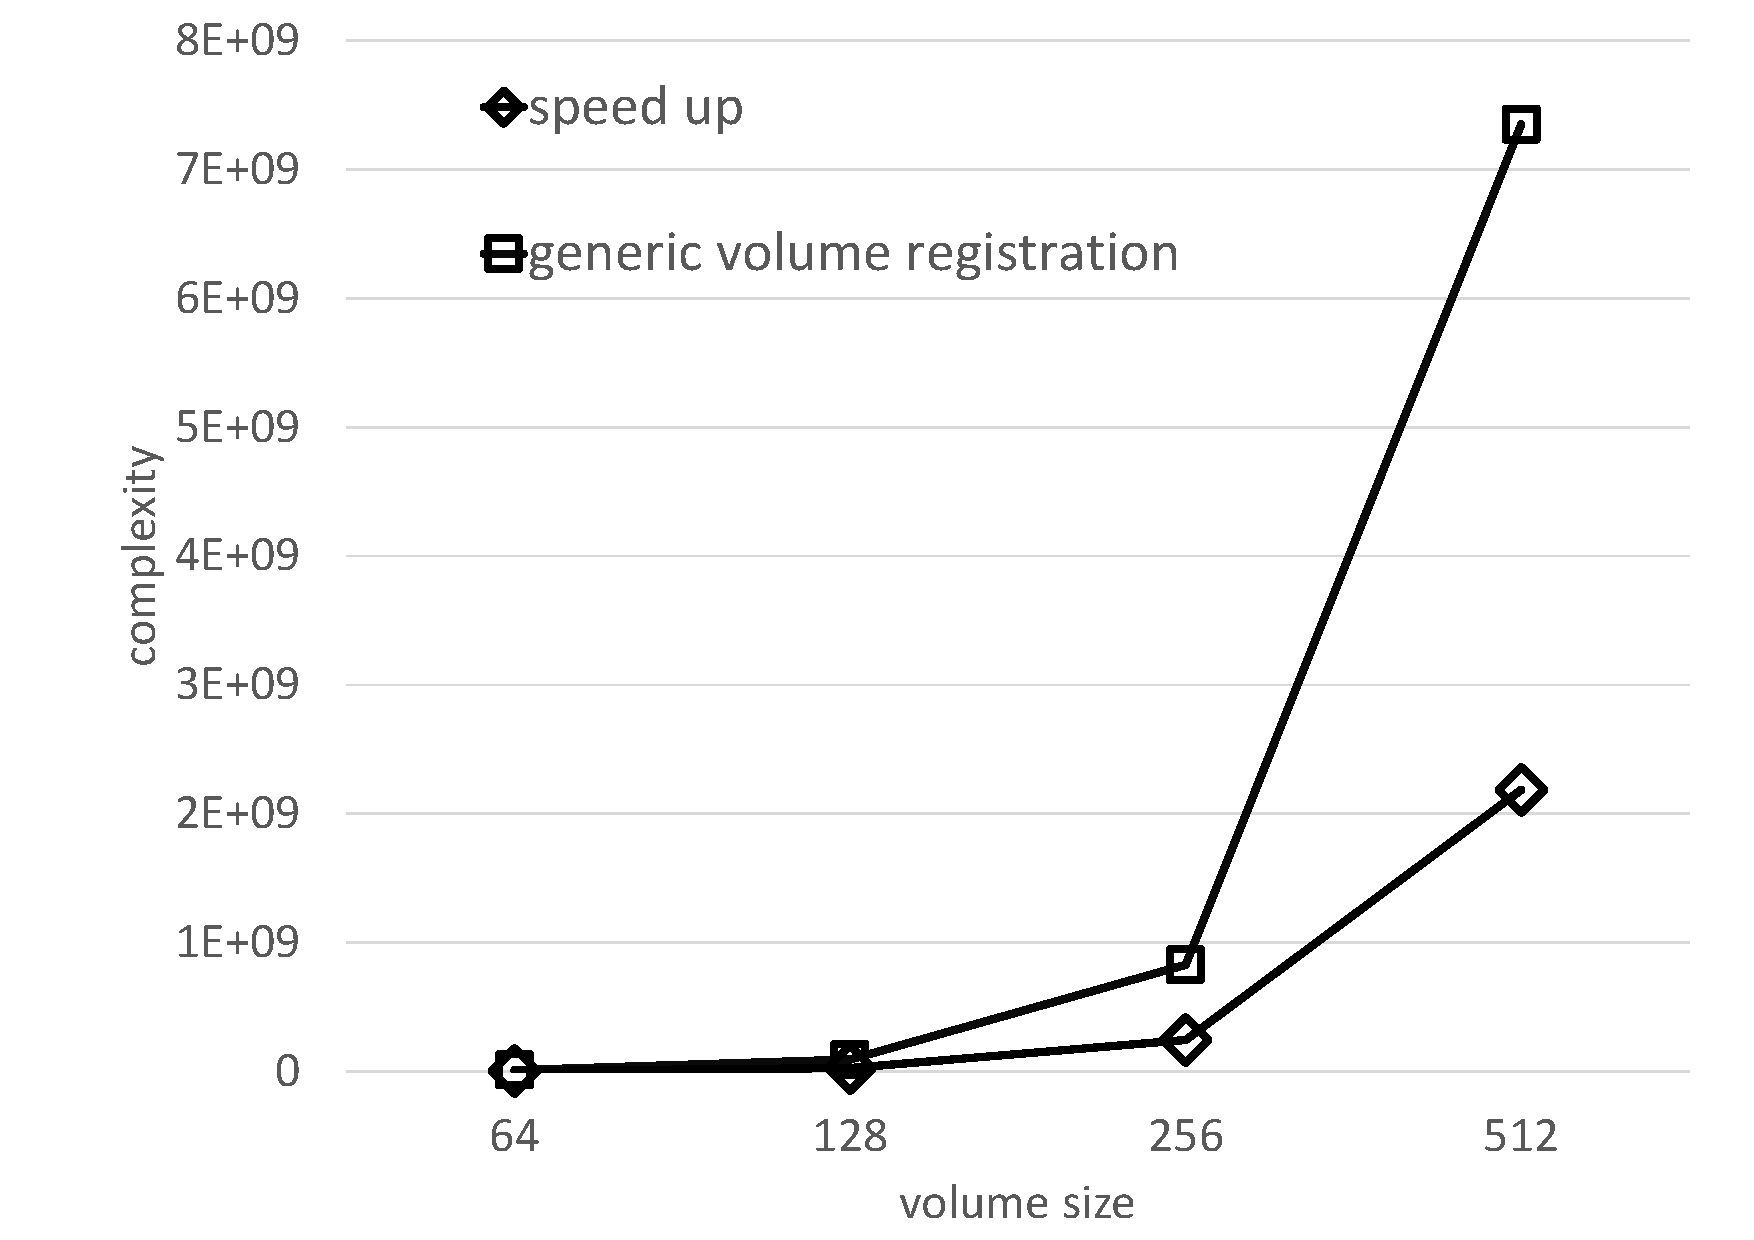
\includegraphics[width=4.0in]{images/ch2/perfcomp}
\caption{Comparison of performance between volume registration and the proposed speed up for different volume sizes.}
\label{fig:perfComp}
\end{figure}



\section{Fourier Volume Registration based 3D Reconstruction}


In this section we describe the general technique of recovering pose estimation via Fourier volume registration techniques. Several methods may be used and each has its own advantages and disadvantages and suitability depends on pose restriction, camera accuracy, noise levels and input data. 


\subsection{A Volume Registration based 3D Reconstruction Pipeline}

\label{METHOD_SECLL}
The proposed 3D reconstruction method consists of various steps. First each frame $f_i$ that is captured, consisting of a colour and depth image pair is projected into 3D space, forming colour point cloud $points_i$ and re-sampled into a volume $V_i$. Then, the transform parameters between pairs of volumes $V_i$ and $V_{i+1}$ are estimated using $VolumeRegister_{\theta \varphi t_x t_y t_z}$ shortened to $VR_{\theta \varphi t_x t_y t_z}$. These parameters are used to update transformation matrix $M$. The points corresponding to $f_2$ ($points_1$) are then transformed using the updated $M$ matrix and added to the cumulative $PointCloud$ database. Two lists, $Cameras$ and $Poses$, are also updated to track camera pose and location per frame. This basic procedure is given in listings \ref{algorithm:PCSLAM} and elaborated upon in subsequent subsections.
\begin{figure}
\begin{lstlisting}[language=c++,caption=Phase Correlation Based SLAM Algorithm,label=algorithm:PCSLAM,mathescape,basicstyle=\ttfamily]
$f_1$ = ReadFrame();
$PointCloud$ = project($f_1$);
$M$ = IdentityMatrix();
$Camera$ = $[0, 0, 0]^T$;
$Pose$ = $[0, 0, 1]^T$;
$Cameras$ = $\left[Camera\right]$, $Poses$ = $\left[Pose\right]$;
while(more frames){
	$f_2$ = ReadFrame();
	$points_1$ = project($f_2$);
	$points_2$ = project($f_1$);
	$V_1$ = ResampleVolume($points_1$);
	$V_2$ = ResampleVolume($points_2$);
	$(\theta, \varphi, t_x, t_y, t_z) = VR_{\theta \varphi t_x t_y t_z}(V_1, V_2)$;
	$M = M \times$TransformMat($(\theta, \varphi, t_x, t_y, t_z)$);
	$points_1$ = Transform($points_1$, $M$);
	$PointCloud$ = $PointCloud \cup points_1$;
	$Camera$ = $M^{-1} \times Camera$;
	$Pose$ = $M^{-1} \times Pose$;
	$Cameras.add(Camera)$;
	$Poses.add\left(\frac{Pose-Camera}{|Pose-Camera|}\right)$;
	$f_1$ = $f_2$;
}
\end{lstlisting}
\end{figure}


The input to our method is a color and depth image pair, $f(u,v)$ and $g(u,v)$ obtained using an Asus Xtion PRO LIVE sensor at a resolution of $640 \times 480$. Each pixel is projected into 3D space using $X_{u,v} = \frac{(u - c_x)Z_{u,v}}{f}$, $Y_{u,v} = \frac{(v - c_y)Z_{u,v}}{f}$ and $Z_{u,v}$ = $g(u,v)$. 
Here, $[c_x c_y]^T$ represent the center of the image whilst $f$ represents the focal length, defined as $525.0$. The point clouds generated by projecting these images are then quantized into image volumes. Results reported in this paper were obtained using volumes of $384^3$ voxels in size.

\begin{figure*}[t]
\centering
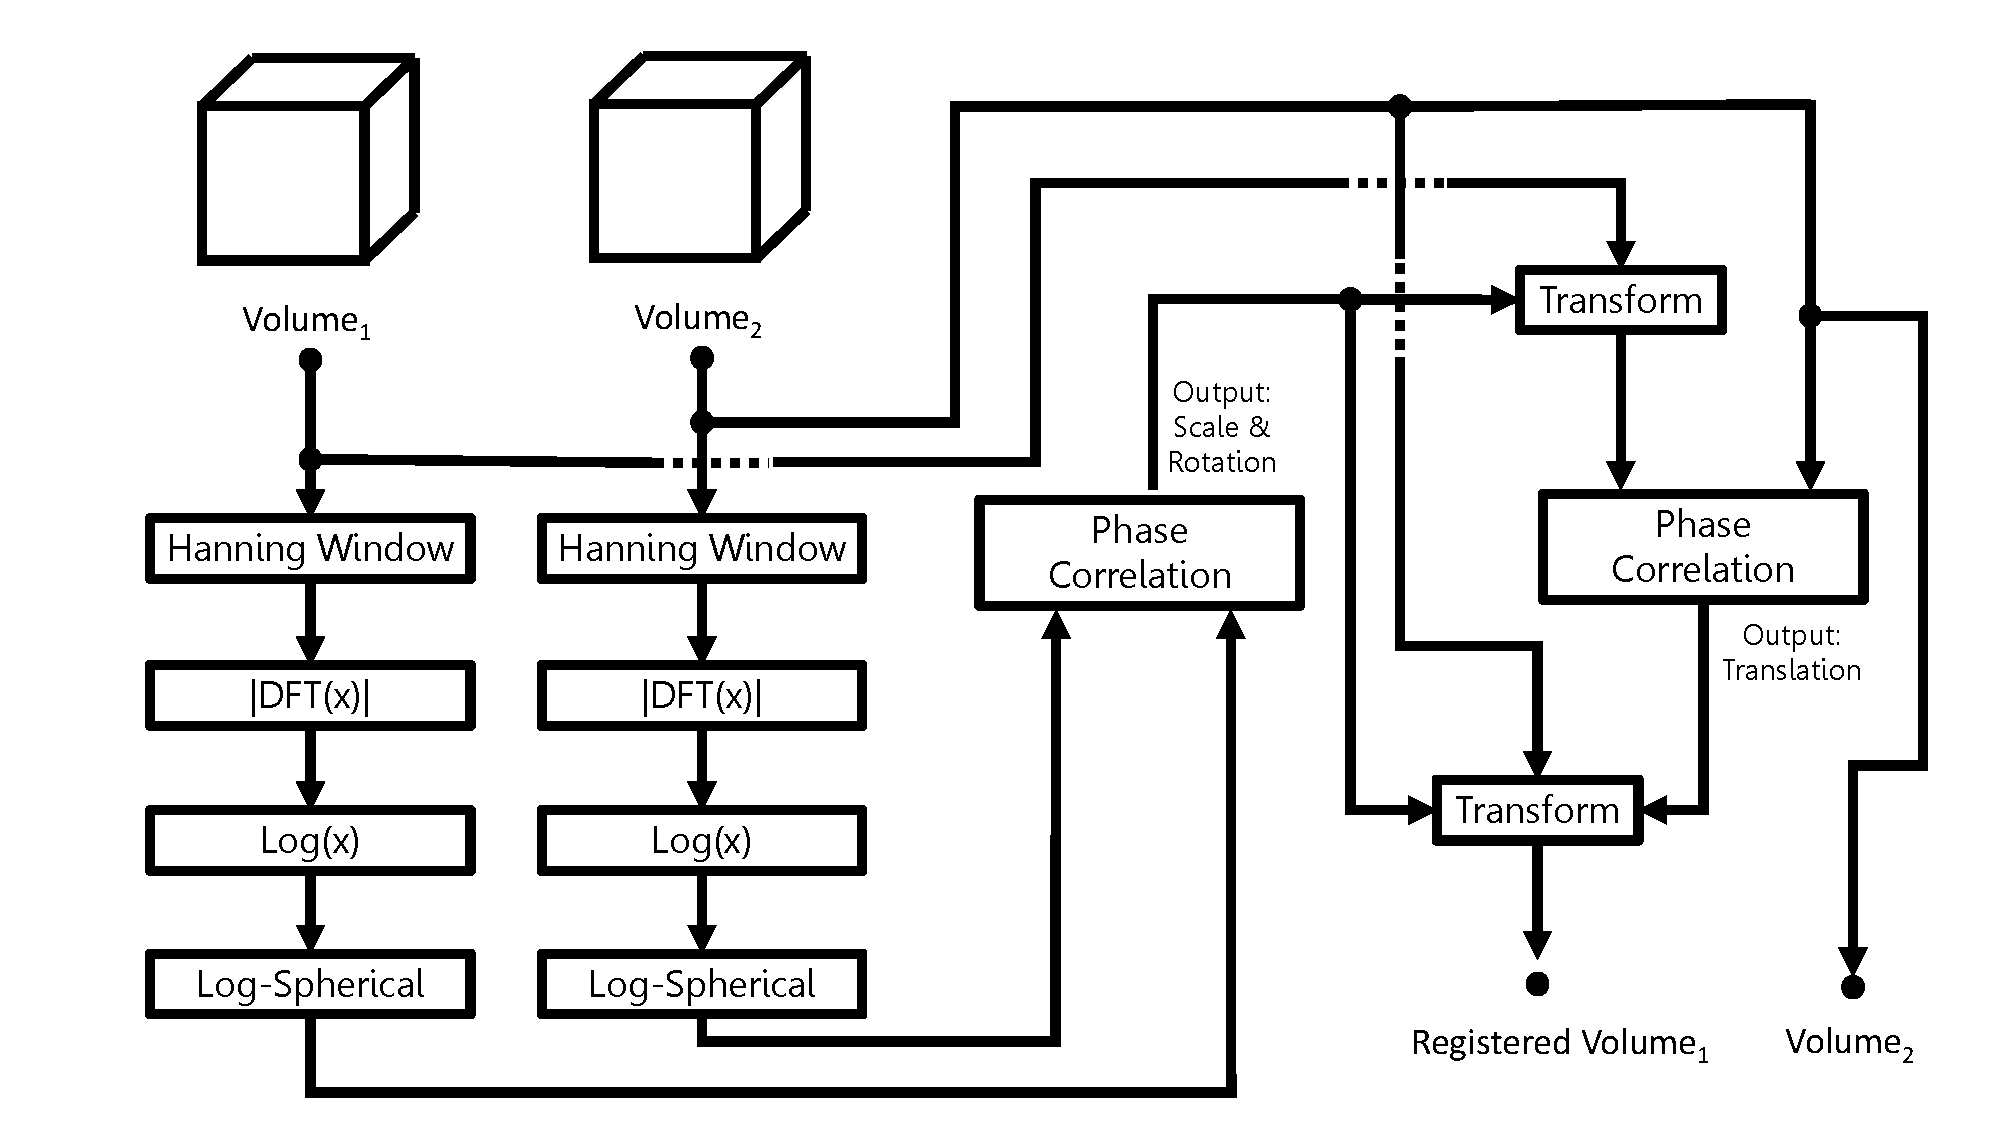
\includegraphics[width=6.0in]{images/ch2/pipeline2}
\caption{System Diagram for Registration Process}
\label{fig:PIPELINE}
\end{figure*}


\subsection{Error metrics}

In order to evaluate the accuracy of volume registration we use several error metrics including: Hausdorff error, mean squared error and the percentage of matched voxels. We describe mathematically those techniques here. All measurements are based on a simple function which computes the nearest neighbour for a given 3D point or voxel given a volume (or collection of 3D points). We define such a function, named nearest-neighbour in equation \ref{eqn:NN}.

\begin{equation} \label{eqn:NN}
NN(p, V) =  \{ q \in V | (Dist(q, p) < Dist(k, p))  \forall k \in V \}
\end{equation}

This function retrieves the closest corresponding point given a query point $p$ and a volume or point cloud of points, $V$. This function can be used to provide omni-directional error functions based on Hausdorff, mean squared and percentage accuracy error metrics.

Here some one-way error functions are described. The one was Hausdorff error is defined in \ref{eqn:HDOW} 

\begin{equation} \label{eqn:HDOW}
\sum_{k=0}^{N} Dist(P_k, NN(P_k, Q))
\end{equation}

\subsection{Reconstruction Integration}

Using the techniques of registration described in the above sections, there are several techniques which may be used to integrate these registered data. In most experiments we use the volume integration to combine the registered data in a single global model. We also propose several techniques for data representation and evaluate their abilities (see section \ref{sec:3DDataRepresentations}). As for the typical volume integration used, we create volumes with dimensions of $512\times 512\times 512$, although larger sizes may be used for increased accuracy. Once a frame is registered, it is projected into the volume. \\

This projection follows the following formula


\begin{equation} \label{eqn:volIntegration}
\begin{split}
x^{1} & = floor((x - frameCenter_x) \times scalar + volumeCenter_x) \\
y^{1} & = floor((y - frameCenter_y) \times scalar + volumeCenter_y) \\
z^{1} & = floor((z - frameCenter_z) \times scalar + volumeCenter_z)
\end{split}
\end{equation}

$frameCenter$ is the center of the projected frame space and $volumeCenter$ is the center of the integration volume, typically scalar is set to 1 or is used to trade-off resolution and map size. An example of an integration process is illustrated in figure XFDF. 


\subsection{Advantages and Disadvantages}





\section{3D Reconstruction Data Representation}
\label{sec:3DDataRepresentations}
In this section we introduce two data representations for recording 3D reconstructions. These novel representations are based on the Octree method. The representations are both designed to compress the data. These methods are inspired by the Shade-Tree and Interpolated Leaf Quad-Tree representations \cite{Gonzalez07ShadeTree, Lincoln13Interpolating} which are used for image compression. These techniques make use of Quad-Tree decomposition and have been shown to outperform several transform based methods of compression. 

\subsection{Octree Decomposition}

In this section we explain Octree decomposition. This strategy forms a cube shaped space around some 3D volumetric data. A data representation is then computed using the location and size of the cube. A measurement system is used to decide if the current data representation fits the data within the cube well or not. If so, then the data representation is used instead of the data. If not, the cube is broken down into 8 sub-cubes and the process is repeated. At each level of decomposition, the data representation achieves finer detail, but more nodes must be stored which means less compression. An example of the Octree is illustrated in figure [INSERT IT HERE].


\subsection{3D ShadeTree Coding}

The Shade-Tree compression system CITE HERE, was designed for the compression of 2D image data. However, this method is easily extended to 3D Volumetric data. In this system, octants are decomposed in the same manner as with a regular octree but the leaf node representation is different. In the Shade-Tree, the corner values in the volume are sampled for each node. Figure XXXXFFG shows an example of these corners given an Octree. The corner values are stored instead of the data within the cube. \\


The actual data representation is formed by interpolating between these 4 corner values to generate the data within the node. This representation saves space by storing 4 corner values only rather than the dense volumetric data. The method also boasts the ability for nodes to share data. For example, if two leaf nodes happen to share a corner we can simply encode the corner once using another data structure at the decompression stage at no cost to the representation. This is illustrated in figure FEFEEF. \\

This data representation may also be used to represent Signed Distance Functions, which are now commonly used in 3d reconstruction as a means of representation. In fact, such a scheme would greatly benefit the compression method of the Shade-Tree since its data is typically represented as smooth changes along a given path. 

\subsection{PlaneTree Coding}

Our method is based on octree subdivision, it begins by placing the mesh within a cube. It checks whether the the representation corresponding to this single cube is at a desired level of quality. If it is not, the cube is decomposed into 8 sub-cubes. For each sub-cube associated with the mesh, the process repeats. This process is typically controlled using an error threshold and a maximum depth value. At each level of subdivision, the error between the sub-cube (or node) representation of the space is compared to the part of the model within the cube. If the error is below the error threshold, decomposition stops. Likewise, if the level of subdivision is greater or equal to the maximum depth value, decomposition also stops. \\

In the typical octree node representation, the raw cube is used to represent the space. Unless this cube is small (deep within the tree) the error is typically high. Trees which are very deep require more storage space. Our method stores arbitrary first order planes within nodes at 20 bits per leaf. This small bit cost per leaf node greatly improves compression performance compared to the octree and makes it competitive with state of the art methods. \\

 
In the following sections, we present the details of the Plane-Tree in terms of subdivision, leaf node plane computation and representation as well as compression and decompression.


\subsection{Octree Subdivision}

Prior to compression, the input 3D model is normalized into a $512^3$ space. Starting with the cube which represents this space, we compute our 3D plane representation. Then the mean squared error between the sampled points of the plane and the sampled points of the model (which lie within the cube) is computed. If this value is below a given threshold, or the maximum level of subdivision is reached, decomposition stops. Alternatively if both of these predicates are not met, the cube is divided into 8 sub-cubes. Each sub-cube is then tested to see whether part of the mesh lies within it. If so, the process it repeated for that cube, otherwise no action is taken. \\

Each cube/sub-cube is referred to as a node. Each node which has no children is referred to as a leaf node. During compression/decompression, our plane based representation is only stored at leaf nodes, with non-leaf nodes serving only as paths giving the location of leaf nodes. Below, the computation and representation of our novel leaf node representation is discussed. \\

\subsection{Leaf Node Computation and Representation}
\label{NRep}
Our novel leaf node representation better represents the mesh which intersects it compared to the octree, it does so by using a first order plane. This representation requires only 20 bits, allowing us to achieve higher quality models whilst saving on bits which would otherwise be used to form a deeper, and thus more costly octree representation. It also gives our method an advantage at low bitrates. \\

In order to generate a plane for a given leaf node, we first sample the mesh within the node space. Using these points, the x, y and z axis variances are measured. These indicate how much variation lies across each axis within the node. We then find the plane using least squares, solving for the axis with the lowest variance. Once we have coefficients describing the plane, we use a single point on the plane, and the plane normal to describe it. \\

Using a point on the plane and a plane normal, we can find a set of triangles which represent the plane within the node. We first find all points in which the cube's edges intersect with the computed plane. Using the average point as the origin, and the plane's normal as the y-axis, we order the points based on their x/z angle. This gives us an ordered set of points which corresponds to a polygon defining the plane within the node. This polygon is then triangulated forming the final representation. This process is used at both the compression and decompression stages. \\

The triangles representing the plane within the node are then sampled along with the parts of the mesh lying within the node. The mean squared error (mse) is then taken between these samples for comparison with the error threshold value. Within the summation for the mse we use the closest point within the second point set, this is shown in equation \ref{eqn:MSE_1}.

\begin{equation}
 \label{eqn:MSE_1}
MSE(pts_1, pts_2) = \frac{1}{N}\sum_{i=0}^{N} (pts_{1_i} - closest(pts_{1_i}, pts_2))^2
\end{equation}

Using this equation and the sampled points from the plane triangles $p$, and the sampled points from the mesh $m$ (which lie within the cube), we take the average of both mean squared errors as a measurement of total error, $error = \frac{1}{2}MSE(p,m) + \frac{1}{2}MSE(m,p)$. This is the value which is compared with the error threshold to decide whether decomposition should stop or not. \\

In order to compress the data for our leaf node representation, we store the the plane using its normal vector and a single point lying on the plane. We store the normal vector using 12 bits (4 bits per coordinate). The point which lies on the plane is represented using two pieces of information, an edge number and a distance variable. First it must be mentioned that for a given plane which intersects a cube, a minimum of 3 of the cube's edges pass through the plane. We therefore record one of these edges (the edge number) and the distance from on of its end points (the distance variable). Each edge has a predefined number which identifies it, all edges also have a predefined start and end point. \\

Each cube has 12 edges in total, so 4 bits are used for the edge number, another 4 are used for the distance variable. Adding these to the normal vector totals to 20 bits per leaf node representation.  \\


\subsection{Compression and Decompression}

In order to compress our data structure we iterate through the tree in depth first order. If we encounter a non-leaf node, we first store a single bit of $1_2$. Then the configuration of the sub-nodes (since not every sub-node intersects the object) is stored as a single byte. Each bit is labelled $1_2$ if a particular sub-node exists and $0_2$ if it does not. This is possible since we order our sub-nodes in a predefined order. If a leaf node is encountered, we store a $0_2$, then record our 20 bit leaf node representation in three other files. One for the normal data, the distance variables and edge numbers totalling 4 files (tree, normals, distances and edge numbers). After the entire structure is stored we employ entropy encoding on each of these files. \\

In order to decompress our structure, we read the first bit of the output file. This checks if the current node is a leaf or not. If it is, we read out a 20 bit plane representation (from the three separate files) and generate a list of triangles representing where the plane intersects the node (explained in section \ref{NRep}). These triangles are then added to a final database which represents the decoded model. If we reach a non-leaf node, we read out the 8 bit sub-node configuration and repeat the process for each existing sub-nodes in the predefined order. \\  


\section{Sensor Input Techniques}


\subsection{Depth Sensor Based Reconstruction}

In this section we describe the process of projecting, registering and integrating 3D reconstructions from depth sensor based input. Depth Sensor based input is fast and reliable but such date not only requires specialized hardware, it also has several draw-backs discussed here. One drawback is that accuracy is limited by the resolution of the device. This means if the application requires higher resolution (more than the standard $640\times 480$) another technique (possibly based on stereo cameras of higher resolution may be required). Another drawback is that certain materials reflect infra-red light, meaning their depth/structure cannot be computed. Salient points within an image typically occur at the edges and corners of objects, these locations however, are known to produce noisy depth information at these pixel locations. \\

A major reason to choose depth sensor based reconstruction frameworks is the consistency and speed of depth data input. For scenes which are easily scanned by depth sensors, this sensor type is typically a preferred choice. A useful sensor input for 3D Fourier Volume Registration includes a color and depth image pair, $f(u,v)$ and $g(u,v)$ respectively. In our experiments, these are obtained using an Asus Xtion PRO LIVE sensor such that $u \in \{0..639\}$ and $v \in \{0..479\}$. Examples of these images are shown in figures \ref{fig:COLEXAMPLE} and \ref{fig:DEPTHEXAMPLE}. Using $Z_{u,v}$ = $g(u,v)$, $f(u,v)$ is projected into 3D space using equation \ref{eqn:PC_PROJECTION} to obtain the $X_{u,v}$ and $Y_{u,v}$ coordinate values in 3D space. Here, $c_x$ and $c_y$ represent the intersection point where the optical axis intersects the projection plane and are defined as $c_x = 319.5$, $c_y = 239.5$. Also $f_x$ and $f_y$ represent the focal length which is defined as $f_x$, $f_y = 525.0$. \\


\begin{equation} \label{eqn:PC_PROJECTION}
\begin{split}
X_{u,v} & = \frac{(u - c_x)Z_{u,v}}{f_x} \\
Y_{u,v} & = \frac{(v - c_y)Z_{u,v}}{f_y} \\
\end{split}
\end{equation}

\begin{figure}[t!] 
        \centering
        \begin{subfigure}[b]{1.8in}
                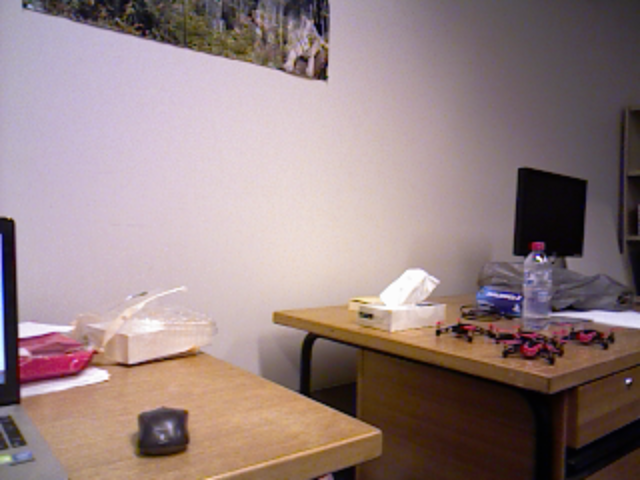
\includegraphics[width=1.7in]{images/ch2/colorF11}
                \caption{Color Image}
                \label{fig:COLEXAMPLE}
        \end{subfigure}%
        \begin{subfigure}[b]{1.8in}
                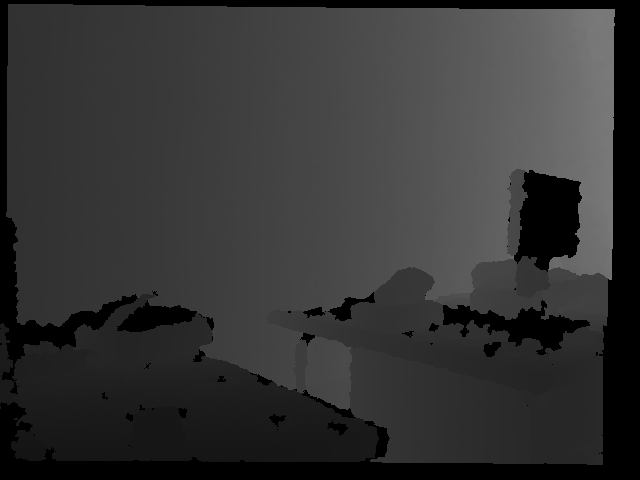
\includegraphics[width=1.7in]{images/ch2/depthF11}
                \caption{Depth Image}
                \label{fig:DEPTHEXAMPLE}
        \end{subfigure}
        
         \begin{subfigure}[b]{1.8in}
                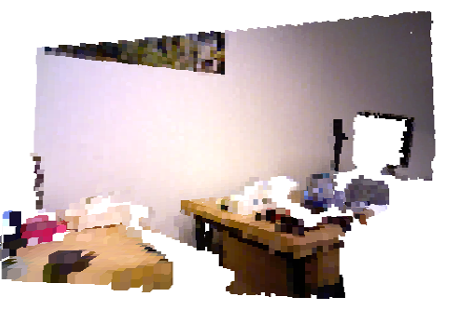
\includegraphics[width=1.8in]{images/ch2/volumeF11128}
                \caption{Projected Volume $128^3$}
                \label{fig:VOLUMEEXAMPLE128}
        \end{subfigure}%
         \begin{subfigure}[b]{1.8in}
                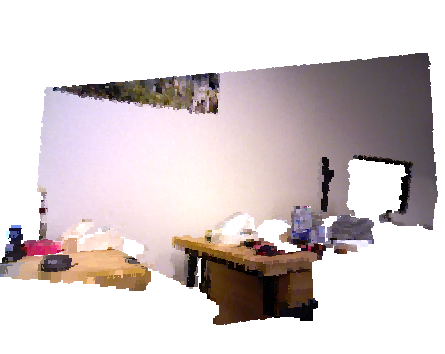
\includegraphics[width=1.8in]{images/ch2/volumeF11256}
                \caption{Projected Volume $256^3$}
                \label{fig:VOLUMEEXAMPLE384}
        \end{subfigure}%
       \caption{A Projected Frame.}
       \label{fig:PROJECTED_FRAME}
\end{figure}


To facilitate further processing, the projected image volumes are re-sampled. The results reported in this paper were obtained using volumes of $256^3$ voxels in size. An example colour and depth image pair and their volumetric projection is shown in figure \ref{fig:PROJECTED_FRAME}.  \\


\subsection{Stereo Camera Based Reconstruction}

The Fourier volume registration methods also work with stereo camera based data. This information can be generated using several of the techniques described in the literature review. Essentially the data must then be projected into depth frames which are registered using one of the proposed fourier volume registration techniques. Because stereo methods do not always accurately compute depth to scale, fourier volume registration has an advantage over other methods in that it also registers against scale. For systems where depth is estimated accurately (as accurately or more than depth sensors) results should work similarly.

\subsection{Monocular Sensor Based 3D Reconstruction}

Some preliminary research has been conducted in evaluating the use of Fourier volume registration given monocular data. From monocular video frames, depth was first computed. This data was fed into the fourier volume registration method in computing 3D reconstructions. Preliminary results are presented but further investigation is required in this area.



\section{Conclusion} % Methodology
\begin{savequote}[8cm]
  ``I just wondered how things were put together.''
  \qauthor{Claude Shannon}
\end{savequote}
\makeatletter
\chapter{Experiments and Results}

\section{Experiments}

This section discusses the types of experiments performed. First, a survey on codec evaluation and comparison techniques is presented, then those techniques used to evaluate the SOT are reported. Next, the experiment environment used is discussed, along with the data set used in experiments.

\begin{figure*}[t] 
        \centering
        \begin{subfigure}[b]{2.0in}
                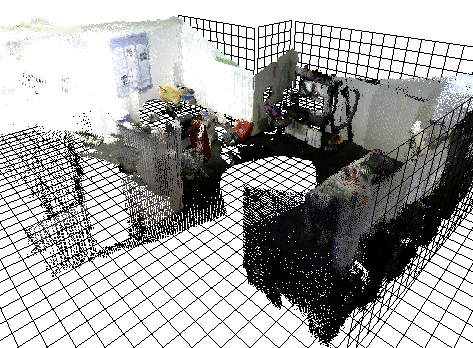
\includegraphics[width=2.0in]{images/ch2/unit21}
                \caption{Apartment}
                \label{fig:RECON_UNIT}
        \end{subfigure}%
        \begin{subfigure}[b]{2.0in}
                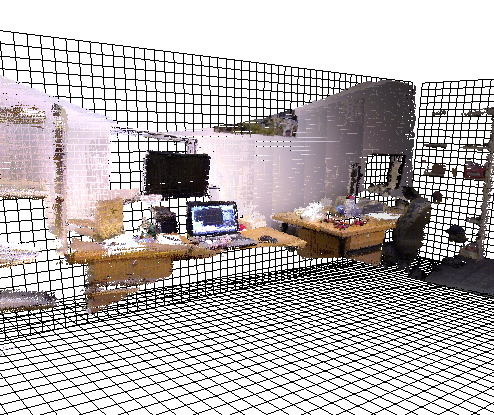
\includegraphics[width=2.0in]{images/ch2/officeA}
                \caption{Office}
                \label{fig:RECON_OFFICE}
        \end{subfigure}%
        \begin{subfigure}[b]{2.0in}
                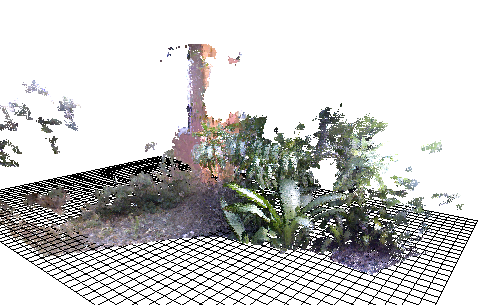
\includegraphics[width=2.0in]{images/ch2/outdoorA}
                \caption{Garden}
                \label{fig:RECON_GARDEN}
        \end{subfigure}
       \caption{Reconstructed Scenes.}
       \label{fig:RECONSTRUCTIONS}
\end{figure*}


\subsection{Codec Evaluation \& Comparison Techniques}

Codec evaluation involves comparing storage requirements between the original model and codec output. In the case of lossy codecs, a quantitative quality metric is also required. Compression metrics are easy to compute, quality metrics are more involved and there have been many proposed techniques. Quality metrics compare the distortion created by the codec relative to the original model. Two measurements are usually performed, the distance from the compressed model to the original and the distance from the original to the compressed model. Quality metrics are split into empirical and perceptual based metrics. Empirical metrics measure geometric error and perceptual metrics estimate human perception. Perception based metrics are a part of psychophysics research. For a more in-depth survey of these methods, see work by Bubill \textit{et al.} \cite{Bulbul11Assessing}.

\subsubsection{Compression Metrics}

In the context of 3D model compression, the file size of both, the compressed model and the original are compared. Alternatively, the file size of the compressed model from one codec can be compared to the file size of the same model compressed using another codec. The compression ratio ($CR$), defined as the original file size divided by the compressed file size, is a measure of compression performance. Another metric used is called the bit rate, different bit rates are used depending on the representation being compressed. The mesh representation uses bits per vertex (bpv) and bits per triangle (bpt), the volumetric representation uses bits per voxel and the point cloud representation uses bits per point.

\subsubsection{Empirical Error Metrics}

The following metrics are used to assess the error between two data samples. For two points, $p$ \& $q$, in $\Re^3$ space, the basic euclidean distance metric,
$$
ED(q,p) = \sqrt{(q_x - p_x)^2 + (q_y - p_y)^2 + (q_z - p_z)^2}
$$,
the absolute error,
$$
AE(q,p) = \|q_x - p_x\| + \|q_y - p_y\| + \|q_z - p_z\|
$$
and the squared error $SE$, 
$$
SE(q,p) = (q_x - p_x)^2 + (q_y - p_y)^2 + (q_z - p_z)^2
$$
are often used as a basis for other metrics. 3D models can be sampled into a set of points in $\Re^3$. Using these samples, the following metrics can be used: sum of distances ($SOD$), sum of absolute differences ($SAD$), sum of squared errors ($SSE$), mean square error ($MSE$) and root mean square error ($RMS$). Since the two models may be sampled differently, the minimum error from one sample to the others is used. These metrics are defined below using two point sets, $A$ \& $B$ where the length of these sets is $M$ and $N$ respectively.
$$
SOD(A,B) = \sum_{k=0}^{M} \min_{b \in B}(ED(A_k,b))
$$

$$
SAD(A,B) = \sum_{k=0}^{M} \min_{b \in B}(AE(A_k,b))
$$

$$
SSE(A,B) = \sum_{k=0}^{M} \min_{b \in B}(SE(A_k,b))
$$

$$
MSE(A,B) = \frac{1}{M}SSE(A,B)
$$

$$
RMS(A,B) = \sqrt{MSE(A,B)}
$$

For each of these metrics, $METRIC(A,B) \neq METRIC(B,A)$. Therefore, these methods are often averaged (below). This is termed the average metric (AM), as opposed to the minimum metric (MM) which is the smallest value of the two.

$$
AvgError = \frac{Metric(A,B)+Metric(B,A)}{2}
$$

Another metric, the Hausdorff distance ($HD$) is a measure of overall shape similarity. It is defined as the largest value of the maximum distances between objects from $A$ to $B$ and from $B$ to $A$. For example, for two objects $A$ \& $B$, the Hausforff distance $HD$, from $A$ to $B$, is defined as,
$$
HD(A,B) = \max(D(A,B),D(B,A))
$$
where $D(A,B)$ is defined as,
$$
D(A,B) = \{a \in A \| \max(dist(a,B)\}
$$
and $dist(a,B)$ is defined below.
$$
dist(a,B) = \{b \in B \left| \min(\|a-b\|)\right.\}
$$

\subsubsection{Human Perception Based Metrics}

Lavoue \textit{et al.} \cite{Lavoue06Perceptually} devised a metric based on structural distortion, this method correlates well with human perception. It is based on the SSIM method of Wang \textit{et al.} \cite{Wang04Image}, which is a popular image metric. Lavoue \textit{et al.} call their method the, Mesh Structural Distortion Measure (MSDM). An updated version of this metric was also developed \cite{Lavoue11Multiscale}.

\paragraph{Laplacian Metric}

Karni \& Gotsman \cite{Karni00Spectral} developed their own on-line metric for use during their spectral based codec. It is based on the laplacian and measures the difference between two objects in terms of their smoothness. 

\paragraph{Elastic Deformation Based Metric}

Bian \textit{et al.} \cite{Bian09Evaluation} developed a novel metric, useful for both on and off-line model comparison. The algorithm is based on the theory of strain fields. A strain field is a metric derived from elasticity, it is used to describe the deformation of some object which has elastic properties. Using this concept, both models are treated as having elastic properties in order to perform quality assessment.

\paragraph{Saliency Based Metrics}

Howlett \textit{et al.} \cite{Howlett04Experimental} and Lee \textit{et al.} \cite{Lee05Mesh} both presented work aimed at determining salient features in 3D models. They incorporated these findings in their own metrics. Howlett \textit{et al.} used a human gaze detection device to study the psychophysical effects of viewing 3D objects. Both of these metrics are based on preserving the sections of the object in which any distortion would be visibly noticeable to humans.

\paragraph{The Depth Difference Metric}

Krivokuca \textit{et al.} \cite{Krivokuca12New} developed a perceptual based metric for the off-line quality assessment of 3D models. This method is independent of model representation and is based on generating multiple depth maps from different orthographic perspectives. It improves upon both the Hausdorff distance and RMS error and is good at detecting both small and large geometric errors. Krivokuca \textit{et al.} call their method, the Depth Difference (DD). It works by comparing orthographic depth maps from both the original and compressed models. First a difference depth image is calculated ($DDI$) from orthographic depth maps of the original object ($DIO$) and of the compressed object ($DIC$). The $DDI$ is calculated using element-wise matrix subtraction,

$$
DDI = DIO - DIC
$$

Then the average depth distance value ($ADD$) is calculated from the $DDI$ matrix, this equation is presented below.

$$
ADD = \frac{1}{MN} \sum_{y=0}^{M} \sum_{x=0}^{N} DDI_{y,x}
$$

This $ADD$ value is then summed up and averaged over different orthographic views, this average is the Depth Difference.

\subsection{Codec Performance Assessment}

The experiments performed use a number of different metrics to quantify the performance of the SOT and compare it with other codecs. The quality metrics used include: mean distance, $RMS$, Depth Difference ($DD$), $MSE$, and qualitative perception. Most research uses the $MSE$ and $RMS$ because they are simple and provide an accurate measurement of quality. Since the data which the SOT is manipulating was designed for human visual consumption, the perceptual metric, DD is used. Our implementation of the DD metric uses five orthogonal projections corresponding to the sides of a cube (excluding the bottom face). Qualitative comparisons are also used to provide insight into the visual quality of the models which the SOT produces. The storage metrics used include: number of bytes and bpv. Bits per vertex is used most often because the input and output of the SOT is a polygonal mesh, and because it is widely used in the literature as part of rate-distortion graphs.

Results provided for the OT use the MM and results for the SOT use the AM. This is because the SOT can represent both outside and inside views of the mesh, whilst the OT can only represents the outside view. All measurements are computed using a $512 \times 512 \times 512$ bounding box, but when comparing the SOT with other codecs, the error is converted to the same bounding box used by the other codec.

\subsubsection{The Metro Program}

In order to ensure the accuracy of geometric errors, the Metro software tool is used to independently assess the quality of models produced by the SOT. This tool takes two models as input and produces the forward and backward $RMS$, mean distance and Hausdorff distance between the two. Metro Version 4.06 was used in all experiments, details about this software can be found in work by Cignoni \textit{et al.} \cite{Cignoni98Metro}.

\subsection{Experiment Environment}

All experiments were performed on an ASUS computer with an Intel i5 CPU and 4 GB of RAM, this machine was running Windows 7. The SOT and OT were written in C++ using Microsoft's Visual Studio IDE, and OpenGL was used to provide visualizations of all models.

\subsection{Data Set}

Industry standard models are used to evaluate the SOT. Six widely used 3D models are used in experiments. These models contain relatively large amounts of geometric information making them a challenge for compression. Figure \ref{dataset} presents this data set. For each model the name, vertex and triangle count are given. With the exclusion of the ball model, these models are commonly used in compression and simplification research. This data set was obtained from the Georgia Institute of Technology's Large Geometric Models Archive \cite{LargeGeometricModelsArchive}. The ball model is included in experiments to provide insight into the compression of smaller 3D models. 


\subsection{Shade-Octree Experiments}

Some experiments are performed on the SOT for the sole purpose of evaluating the best LOD and distance code search length (DCL) to use. Since these variables directly affect he SOT's efficiency, experiment results are provided. Both of these experiment types are described in detail below.


\subsubsection{Distance Code Length Tests}

The SOT makes use of four distance codes per node. These distance codes are truncated to a multiple of the node's region size. This multiple is called the distance code length (DCL). To evaluate the optimal DCL, six sets of experiments are performed, each using DCL values ranging from one to six. For each experiment, $MSE$ threshold values of: $1$, $16$ and $512$ are used, these provide rate-distortion curves for each DCL experiment. In these experiments, the bunny model is used and both visual and graphical results are presented. This test is important because it reveals the best choice for the DCL. The optimal selection of the DCL may have an impact on codec efficiency. 

\subsubsection{Maximum Level of Depth Tests}

The level of depth (LOD) threshold represents the minimum leaf region size (how far the tree can be decomposed). A smaller LOD provides more accuracy but requires more storage size, a larger code results in a smaller file size with more distortion. To select the best LOD, five experiments are performed using LOD values of: 1, 2, 4, 8 and 16. All results are obtained using the bunny model and both numerical and graphical results are provided. These experiments are performed to find the optimal choice of the LOD threshold, which affects the efficiency of the SOT. 

\subsection{Codec Comparisons}

The SOT is compared with a generic implementation of the OT, as well as other state of the art codecs. These experiments are discussed in the sections below.


\subsubsection{OT Comparison}

The OT algorithm is the main competitor of the SOT, it is a very well known and used 3D compression and representation structure. Rate-distortion curves are used to compare these codecs. In these experiments, $bpv$ is used as the bit rate, and both $DD$ and the $MSE$ metrics are used to measure quality. A qualitative quality analysis is also used to compare the two codecs. 

\subsubsection{State of the Art Comparisons}

The SOT is compared to other codecs which have been shown to have state of the art performance. The method by Peng \& Kuo \cite{Peng05Geometry-Guided} is compared with the SOT using a rate-distortion graph with the rabbit model. The progressive wavelet compression method by Khodakovsky \textit{et al.} \cite{Khodakovsky00Progressive} is also compared using a rate-distortion graph using the bunny model. Both the spectral codec by Karni \& Gotsman \cite{Karni00Spectral} and the state of the art single-rate codec by Touma \& Gotsman \cite{touma98triangle} are compared using a qualitative quality assessment of the bunny model. The hierarchical point-cloud codec by Siddiqui \textit{et al.} \cite{Siddiqui07Octree} is also compared with the SOT using a qualitative analysis. Recent state of the art codecs, including the FOLProM codec by Peng \textit{et al.} \cite{Peng10Feature} and the spectral codec by Bayazit \textit{et al.} \cite{Bayazit103DMesh} are also compared.
 % Experiments &
\section{Results}

This section presents and analyses the results from experiments. The experiments used to evaluate the optimal LOD and DCL values are presented first. Then the SOT is compared with the OT codec and with the current state of the art codecs from the literature. Results include both, rate-distortion and qualitative quality tests. 

\subsection{LOD \& DCL Evaluation}

\subsubsection{Distance Code Length Evaluation}

DCL values tested include $1$, $2$, $3$, $4$, $5$ and $6$. First, rate-distortion graphs are presented, then visual results are discussed.

\paragraph{Rate-Distortion Graphs}

Figure \ref{DistanceCodeRDGraphs} shows the rate-distortion graphs used to evaluate the different DCL values. The graphs in the top row use the $MSE$ metric and the graphs in the bottom row use the depth difference ($DD$) metric. The $MSE$ rate-distortion graphs suggest that DCL values of $5$ and $6$ perform slightly better than the others. The $DD$ rate-distortion graphs show that DCL values of $6$ and $3$ perform better, with $6$ performing well at high bit rates and $3$ performing well at lower to mid level bit rates. Overall, these results do not provide a clear indication of an optimal DCL value but it can be seen that values of $1$ and $2$ do not perform as well as the higher values.


\paragraph{Visual Comparisons}


Two sets of visual comparisons are presented to evaluate the optimal DCL value. Figure \ref{DistanceCodeVisualTests1} shows results at higher bit rates and figure \ref{DistanceCodeVisualTests2} shows results at lower bit rates. Both sets of results suggest that a DCL value of $1$ produces undesirable models with many holes. Results seem to be quite similar for DCL values of $3$ and above. A DCL value of $2$ provides a slight $MSE$ advantage at a higher bit cost, but in both figures, this quality difference is not noticeable.


\paragraph{Conclusion}

Results shown that a DCL value of $1$ produces poor results, both in a rate-distortion and qualitative quality sense. A DCL value of $2$ produces a higher calibre model in the $MSE$ sense, at the expense of a higher bit rate. This $MSE$ quality advantage is unnoticeable in qualitative comparisons, compared to values of $3$ and above. Therefore it is generalized that, DCL values of $3$ and above, are the best choice for use in the SOT.

\subsubsection{Level of Depth Threshold Evaluation}

LOD tests are used to evaluate the optimal choice of LOD threshold. Different LOD threshold comparisons include: $1$, $2$, $4$, $8$ and $16$.

\paragraph{Rate-Distortion Graphs}

Figure \ref{LevelsOfDepthRDGraphs} shows two rate-distortion graphs, the left graph uses the $MSE$ metric and the right graph uses the perceptual $DD$ metric. The $MSE$ graph suggests that an LOD threshold value of $8$ is optimal for higher bit rates and a value of $16$ is best for lower bit rate compression. The $DD$ metric graph suggests that the LOD of $8$ is the optimal threshold value. It produces the best results and is comparable to LOD $16$ even at low bit rates. Both graphs suggest that LOD values of $1$ and $2$ result in poor performance, this is due to the fact that these levels require more branches in the tree, increasing storage requirements. An SOT with a shallow tree that accurately accurately approximates the model is ideal.

\paragraph{Visual Comparisons}


Visual comparisons further provide an indication of the best LOD threshold to use. Figure \ref{LevelsOfDepthVisualTests1} shows high bit rate results using different LOD values, and figure \ref{LevelsOfDepthVisualTests2} shows the same tests for lower bit rates. In figure \ref{LevelsOfDepthVisualTests1}, the bit rate becomes lower and lower as the LOD value is raised, but only on the transition from $8$ to $16$ does this advantage wear off, as the LOD $16$ model is more distorted than the rest. This further suggests that the optimal LOD value is $8$. Figure \ref{LevelsOfDepthVisualTests2} also suggests this conclusion. Notice that with low bit rate compression, the models with LOD values ranging $1-8$ look similar, but $8$ has the lowest bit rate.


\paragraph{Conclusion}

The optimal LOD value is more obvious than the optimal DCL code. Both, rate-distortion graphs and visual results reveal that the optimal LOD threshold is level $8$. Since all models are bound to a $512\times 512 \times 512$ box, where the root node is defined as level $0$, the SOT should be decomposed until a maximum tree depth of $6$.

\subsection{SOT vs. OT Results}

This section presents results comparing the the SOT with the OT. Models tested include: Ball, Bunny, Horse, Rabbit, Dragon, Angel and Happy Buddha. Tabulated results for the SOT are provided in Appendix \ref{AppendixA}.

\subsubsection{Rate-Distortion Graphs}

RD results for the ball model are presented in figure \ref{ballRDGraphs}. The $MSE$ metric graph (left) shows that the SOT outperforms the OT codec, and the $DD$ metric graph supports this conclusion. In the $DD$ graph, the OT cannot reach the quality of the SOT, even at very high bit rates.

Rate-distortion results for the bunny model are presented in figure \ref{bunnyRDGraphs}. These results are similar with those obtained using the ball model. In these results, the SOT outperforms the OT codec. In the rate-distortion graphs for the horse, the $MSE$ metric graph on the left of figure \ref{horseRDGraphs} shows that the OT comes close to the performance of the SOT, but still has worse performance. When considering the same figure where the $DD$ metric is used (right), the SOT produces much better results than the OT.

Rate-distortion graphs for the: rabbit, angel, dragon and happy buddha are shown in figures: \ref{rabbitRDGraphs}, \ref{angelRDGraphs}, \ref{dragonRDGraphs} and \ref{happyRDGraphs} respectively. These results show similar findings in that the SOT is more efficient than the OT codec in terms of rate-distortion, especially in terms of quantitative perceptual quality (DD).

\subsubsection{Visual comparisons}

Visual comparisons make a case for the practicality of the SOT because this data is meant for human visual consumption. In figure \ref{ballVisualResults} the ball is coded with the SOT and OT, the outputs of these codecs are compared with the original model. These results show a large difference in quality between the SOT and the OT. The OT codec produces a blocky, spikey shape which does not correlate with the outline of the original model. The SOT produces a more visually pleasing result whilst using two thirds of the storage requirements of the OT. 


The bunny visual results are shown in figure \ref{bunnyVisualResults}, these results show that for a similar bit rate, the SOT codec produces a higher quality model than the OT. The outline of the SOT coded model looks similar to the original model, but does have some holes. The holes are present because the SOT is rendered directly from the tree structure without being filtered. Despite this, it is still less distorted than the model compressed using the OT. 


Visual results for the horse model are presented in figure \ref{horseVisualResults}. These results show that for a lower bit rate, the SOT codec produces a higher quality model compared with the OT. Results for the rabbit (figure \ref{rabbitVisualResults}) also show that for a lower bit rate, the SOT produces better quality models. In the rabbit results, the SOT coded model looks very similar to the original model whilst the OT coded model is blocky and distorted. It is clear that the OT has suffered from 3D aliasing. 

Visual results for the angel, dragon and happy buddha are provided in figures, \ref{angelVisualResults}, \ref{dragonVisualResults} and \ref{happyVisualResults} respectively. These results show that, at low bit rates, the SOT produces models which fit the outline of the original model better.


\subsubsection{Conclusion}

Results show that the SOT outperforms the OT codec in both, rate-distortion tests and in qualitatively quality analysis. The SOT produces models which match the general shape of the original model well, however some filtering is required to fill infrequently occurring holes. The OT produces models which have aliasing and distortion, plus the OT produces higher bit rates.

\subsection{Comparisons with the State of the Art}

Codecs used for state of the art comparisons include: the progressive mesh OT by Peng \textit{et al.} \cite{Peng05Geometry-Guided}, the wavelet codec by Khodakovsky \textit{et al.} \cite{Khodakovsky00Progressive}, FOLProM by Peng \textit{et al.} \cite{Peng10Feature}, the hierarchical point cloud codec by Siddiqui \textit{et al.} \cite{Siddiqui07Octree}, the valence driven codec \cite{touma98triangle}, the spectral codec by Karni \& Gotsman \textit{et al.} \cite{Karni00Spectral} and the other spectral codec by Bayazit \textit{et al.} \cite{Bayazit103DMesh}. 

\subsubsection{Rate-Distortion Graphs}

Figure \ref{Peng05Geometry-GuidedRDGraph} shows a rate-distortion graph comparing the progressive OT codec by Peng et al. \cite{Peng05Geometry-Guided} with the SOT.  Results show that the SOT outperforms this codec. Results comparing the SOT and the wavelet codec by Khodakovsky \textit{et al.} \cite{Khodakovsky00Progressive} are shown in figure \ref{Khodakovsky00ProgressiveRDGraph}. This graph uses the $MSE$ as the quality metric and the bunny model as codec input. This graph shows that the SOT outperforms the wavelet codec.


Peng \textit{et al.} have another, more recent codec called FOLProM  \cite{Peng10Feature}. Results are shown in figure \ref{Peng10FeatureRDGraph}. The left graph shows results for the dragon, and the right graph shows results for the rabbit model. In both graphs, the SOT has a better rate-distortion curve.

\subsubsection{Visual comparisons}

Figure \ref{SOTSiddiqui07OctreeVisualResults} shows visual results for the SOT and the codec by Siddiqui \textit{et al.} \cite{Siddiqui07Octree}. The two models on the left were compressed by the SOT, the middle model is the original and the models on the right were compressed by the point cloud OT codec. Results show that the SOT requires $2.840$ bpv to represent the original bunny model accurately, whilst the codec by Siddiqui \textit{et al.} requires at least $11.2$ bpv to to store the model at a similar quality level. At $8.3$ bpv their models become slightly distorted, and at $5.8$ bpv, they become very distorted, not reaching the quality of the SOT codec.
 

Figure \ref{SOTtouma98triangleKarni00SpectralVisualResults} shows visual results for the SOT, the valence driven approach \cite{touma98triangle} and the spectral codec \cite{Karni00Spectral}. The first two models are SOT outputs, the center model is the original bunny model, the center right model was produced by the spectral codec and the far right model was compressed using the valence driven approach. The SOT coded models look quite similar to the original model, the SOT model with a bit rate of $1.461$ does look a bit blocky, however it has a much lower bit rate compared with the other models. The far left codec with a bit rate of $3.984$ is similar to the original model but suffers from a missing patch on its left foot, however, the ears and legs correlate well with the original model. The valence driven codec produces undesirable results, its output model is lumpy and is quite distorted. The spectral coded model looks better but looks overly lumpy. The SOT's improvement over the spectral codec is somewhat arguable, but the SOT is a clear improvement over the valence driven approach.


Figure \ref{SOTBayazit103DMeshVisualResults} shows results comparing the SOT with the recent spectral codec by Bayazit \textit{et al.} \cite{Bayazit103DMesh}. At a bit rate of $1.461$, the SOT codec produces a smoother version of the original model, whilst the spectral codec by Bayazit requires $2.523$ bpv to produce a model which is very lumpy and distorted. These results suggest the SOT is the better codec.

\subsection{Conclusion}

Experiments show that the optimal LOD threshold is $8$ and the best DCL values are above or equal to $3$. Results have also revealed that the SOT outperforms both the OT and other state of the art codecs from the literature in terms of rate-distortion and qualitative quality. The hierarchical SOT method produces models which accurately reflect the general shape of the original model and transform based codecs produce models which are lumpy. These results suggest that the SOT is among the current state of the art 3D data compression schemes available.

 % Results
\begin{savequote}[8cm]
  ``Learn from yesterday, live for today, hope for tomorrow. The important thing is not to stop questioning.''
  \qauthor{Albert Einstein}
\end{savequote}
\makeatletter
\chapter{Conclusion}

\section{Research Aims Revisited}

The primary aim of this research was to improve the storage, quantitative quality and perceptual quality of 3D models. Hierarchical methods were investigated and this led to a new image codec, ILQT \cite{Lincoln13Interpolating} as well as the proposed scheme, the Shade-Octree. The research question was, ``Do hierarchical techniques bring state of the art compression performance to 3D data?'' Results from chapter 4 show that the SOT outperforms the OT compression scheme as well as several state of the art methods in terms of rate-distortion and perceptual quality. The primary aim of this research has been accomplished because the SOT produces models which have improved storage efficiency, whilst improving quantitative quality and perceptual quality compared with other compression schemes. The proposed research question can also be answered. The SOT, a hierarchical codec, does achieve state of the art performance in the field of 3D data compression.

\section{Future Work}

There is still much work to be done in the area of hierarchical 3D data compression. One possible project could be to improve the SOT. Currently the SOT can produce holes in the output mesh, an investigation of this may lead to improved results. Other projects could investigate the extension of the PJQ, wedglet, BSP-tree and QB tree to 3D model compression.
 % Conclusion
\appendix
none
%\makeatletter
\chapter{Appendix A}
\label{AppendixA}

\section{Tabulated Results}

\begin{table}[h]
\begin{tabular}[c]{|c|c|c|c|c|c|c|c|c|}
\hline\multicolumn{9}{|c|}{\textbf{SOT Results Using the Ball Graph}}\\
\hline
\textbf{Threshold} & \textbf{LOD} & \textbf{bytes} & \textbf{Mean} & \textbf{RMS} & \textbf{MSE} & \textbf{DD} & \textbf{Hausdorff} & \textbf{bpv}\\
\hline
1 & 8 & 2877 & 0.209 & 0.335 & 0.112 & 1.186 & 9.938 & 47.751\\
\hline
2 & 8 & 2111 & 0.309 & 0.473 & 0.223 & 1.603 & 8.899 & 35.037\\
\hline
4 & 8 & 1517 & 0.448 & 0.657 & 0.432 & 2.287 & 8.269 & 25.178\\
\hline
8 & 8 & 1111 & 0.603 & 0.917 & 0.841 & 4.846 & 21.755 & 18.440\\
\hline
16 & 8 & 928 & 0.674 & 1.036 & 1.073 & 6.052 & 21.755 & 15.402\\
\hline
32 & 8 & 841 & 0.741 & 1.270 & 1.613 & 11.391 & 21.755 & 13.959\\
\hline
64 & 8 & 856 & 0.743 & 1.275 & 1.626 & 11.526 & 21.755 & 14.207\\
\hline
\end{tabular}
\caption{A table displaying results for the SOT using the Ball model}
\label{table:SOTTableBall}
\end{table}

\begin{table}[h]
\begin{tabular}[c]{|c|c|c|c|c|c|c|c|c|}
\hline\multicolumn{9}{|c|}{\textbf{SOT Results Using the Bunny Graph}}\\
\hline
\textbf{Threshold} & \textbf{LOD} & \textbf{bytes} & \textbf{Mean} & \textbf{RMS} & \textbf{MSE} & \textbf{DD} & \textbf{Hausdorff} & \textbf{bpv}\\
\hline
1 & 8 & 6566 & 0.376 & 0.609 & 0.371 & 2.814 & 10.081 & 1.461\\
\hline
2 & 8 & 5475 & 0.482 & 0.744 & 0.554 & 3.005 & 11.532 & 1.218\\
\hline
4 & 8 & 4415 & 0.622 & 0.914 & 0.836 & 3.468 & 11.777 & 0.983\\
\hline
8 & 8 & 3632 & 0.809 & 1.172 & 1.374 & 3.946 & 14.448 & 0.808\\
\hline
16 & 8 & 2945 & 1.061 & 1.513 & 2.290 & 4.805 & 21.251 & 0.655\\
\hline
128 & 8 & 2096 & 1.514 & 2.162 & 4.674 & 7.291 & 21.283 & 0.466\\
\hline
256 & 8 & 1984 & 1.603 & 2.311 & 5.343 & 8.270 & 23.680 & 0.442\\
\hline
512 & 8 & 1878 & 1.673 & 2.442 & 5.964 & 9.163 & 23.680 & 0.418\\
\hline
\end{tabular}
\caption{A table displaying results for the SOT using the Bunny model}
\label{table:SOTTableBunny}
\end{table}

\begin{table}[h]
\begin{tabular}[c]{|c|c|c|c|c|c|c|c|c|}
\hline\multicolumn{9}{|c|}{\textbf{SOT Results Using the Horse Graph}}\\
\hline
\textbf{Threshold} & \textbf{LOD} & \textbf{bytes} & \textbf{Mean} & \textbf{RMS} & \textbf{MSE} & \textbf{DD} & \textbf{Hausdorff} & \textbf{bpv}\\
\hline
1 & 8 & 3349 & 0.469 & 0.731 & 0.534 & 2.778 & 9.523 & 0.553\\
\hline
2 & 8 & 3002 & 0.535 & 0.797 & 0.635 & 2.849 & 9.523 & 0.495\\
\hline
4 & 8 & 2605 & 0.676 & 0.986 & 0.972 & 3.132 & 13.978 & 0.430\\
\hline
8 & 8 & 2218 & 0.886 & 1.251 & 1.564 & 3.416 & 13.978 & 0.366\\
\hline
16 & 8 & 1949 & 1.121 & 1.560 & 2.433 & 4.002 & 16.394 & 0.322\\
\hline
128 & 8 & 1585 & 1.571 & 2.222 & 4.938 & 4.744 & 17.055 & 0.262\\
\hline
256 & 8 & 1516 & 1.669 & 2.385 & 5.689 & 4.922 & 17.055 & 0.250\\
\hline
512 & 8 & 1489 & 1.696 & 2.433 & 5.918 & 5.173 & 17.202 & 0.246\\
\hline
1024 & 8 & 1480 & 1.793 & 2.707 & 7.330 & 5.260 & 27.590 & 0.244\\
\hline
\end{tabular}
\caption{A table displaying results for the SOT using the Horse model}
\label{table:SOTTableHorse}
\end{table}

\begin{table}[h]
\begin{tabular}[c]{|c|c|c|c|c|c|c|c|c|}
\hline\multicolumn{9}{|c|}{\textbf{SOT Results Using the Rabbit Graph}}\\
\hline
\textbf{Threshold} & \textbf{LOD} & \textbf{bytes} & \textbf{Mean} & \textbf{RMS} & \textbf{MSE} & \textbf{DD} & \textbf{Hausdorff} & \textbf{bpv}\\
\hline
1 & 8 & 3041 & 0.389 & 0.572 & 0.327 & 1.405 & 9.438 & 0.363\\
\hline
2 & 8 & 2491 & 0.507 & 0.725 & 0.526 & 1.539 & 9.282 & 0.297\\
\hline
4 & 8 & 2017 & 0.681 & 0.942 & 0.888 & 1.908 & 9.282 & 0.241\\
\hline
8 & 8 & 1592 & 0.901 & 1.225 & 1.501 & 2.225 & 12.738 & 0.190\\
\hline
16 & 8 & 1226 & 1.156 & 1.536 & 2.359 & 2.687 & 12.831 & 0.146\\
\hline
128 & 8 & 810 & 1.680 & 2.275 & 5.176 & 3.684 & 18.271 & 0.097\\
\hline
256 & 8 & 763 & 1.757 & 2.409 & 5.802 & 4.044 & 18.271 & 0.091\\
\hline
512 & 8 & 737 & 1.809 & 2.520 & 6.352 & 4.895 & 20.418 & 0.088\\
\hline
\end{tabular}
\caption{A table displaying results for the SOT using the Rabbit model}
\label{table:SOTTableRabbit}
\end{table}

\begin{table}[h]
\begin{tabular}[c]{|c|c|c|c|c|c|c|c|c|}
\hline\multicolumn{9}{|c|}{\textbf{SOT Results Using the Angel Graph}}\\
\hline
\textbf{Threshold} & \textbf{LOD} & \textbf{bytes} & \textbf{Mean} & \textbf{RMS} & \textbf{MSE} & \textbf{DD} & \textbf{Hausdorff} & \textbf{bpv}\\
\hline
2 & 8 & 3395 & 0.774 & 1.221 & 1.491 & 2.831 & 20.748 & 0.115\\
\hline
16 & 8 & 2487 & 1.092 & 1.620 & 2.624 & 3.097 & 20.748 & 0.084\\
\hline
64 & 8 & 1963 & 1.563 & 2.288 & 5.234 & 3.673 & 20.748 & 0.066\\
\hline
128 & 8 & 1779 & 1.851 & 2.708 & 7.335 & 4.036 & 20.748 & 0.060\\
\hline
\end{tabular}
\caption{A table displaying results for the SOT using the Angel model}
\label{table:SOTTableAngel}
\end{table}

\begin{table}[h]
\begin{tabular}[c]{|c|c|c|c|c|c|c|c|c|}
\hline\multicolumn{9}{|c|}{\textbf{SOT Results Using the Dragon Graph}}\\
\hline
\textbf{Threshold} & \textbf{LOD} & \textbf{bytes} & \textbf{Mean} & \textbf{RMS} & \textbf{MSE} & \textbf{DD} & \textbf{Hausdorff} & \textbf{bpv}\\
\hline
2 & 8 & 6191 & 0.748 & 1.402 & 1.965 & 5.706 & 25.885 & 0.113\\
\hline
16 & 8 & 4617 & 1.044 & 1.746 & 3.049 & 5.935 & 25.885 & 0.084\\
\hline
64 & 8 & 3789 & 1.324 & 2.122 & 4.501 & 6.415 & 25.885 & 0.069\\
\hline
128 & 8 & 3473 & 1.501 & 2.440 & 5.952 & 7.305 & 25.946 & 0.063\\
\hline
512 & 8 & 2957 & 1.795 & 2.898 & 8.401 & 8.330 & 25.946 & 0.054\\
\hline
\end{tabular}
\caption{A table displaying results for the SOT using the Dragon model}
\label{table:SOTTableDragon}
\end{table}

\begin{table}[h]
\begin{tabular}[c]{|c|c|c|c|c|c|c|c|c|}
\hline\multicolumn{9}{|c|}{\textbf{SOT Results Using the Happy Buddha Graph}}\\
\hline
\textbf{Threshold} & \textbf{LOD} & \textbf{bytes} & \textbf{Mean} & \textbf{RMS} & \textbf{MSE} & \textbf{DD} & \textbf{Hausdorff} & \textbf{bpv}\\
\hline
2 & 8 & 4974 & 0.853 & 1.339 & 1.793 & 4.987 & 11.154 & 0.073\\
\hline
16 & 8 & 3953 & 1.068 & 1.640 & 2.690 & 4.983 & 15.687 & 0.058\\
\hline
64 & 8 & 3096 & 1.407 & 2.167 & 4.697 & 5.500 & 15.732 & 0.046\\
\hline
128 & 8 & 2726 & 1.635 & 2.504 & 6.269 & 5.931 & 17.188 & 0.040\\
\hline
\end{tabular}
\caption{A table displaying results for the SOT using the Happy Buddha model}
\label{table:SOTTableHappy}
\end{table}
 % Appendix A
\backmatter
\openup -0.5em
%\bibliographystyle{plain}
\bibliographystyle{IEEEtran}
\bibliography{bibliographies/slam,bibliographies/compress}
\end{document}